%%%%%%%%%%%%%%%%%%%%%%%%%%%%%%%%%%%%%%%%%
% The Legrand Orange Book
% LaTeX Template
% Version 2.0 (9/2/15)
%
% This template has been downloaded from:
% http://www.LaTeXTemplates.com
%
% Mathias Legrand (legrand.mathias@gmail.com) with modifications by:
% Vel (vel@latextemplates.com)
%
% License:
% CC BY-NC-SA 3.0 (http://creativecommons.org/licenses/by-nc-sa/3.0/)
%
% Compiling this template:
% This template uses biber for its bibliography and makeindex for its index.
% When you first open the template, compile it from the command line with the 
% commands below to make sure your LaTeX distribution is configured correctly:
%
% 1) pdflatex main
% 2) makeindex main.idx -s StyleInd.ist
% 3) biber main
% 4) pdflatex main x 2
%
% After this, when you wish to update the bibliography/index use the appropriate
% command above and make sure to compile with pdflatex several times 
% afterwards to propagate your changes to the document.
%
% This template also uses a number of packages which may need to be
% updated to the newest versions for the template to compile. It is strongly
% recommended you update your LaTeX distribution if you have any
% compilation errors.
%
% Important note:
% Chapter heading images should have a 2:1 width:height ratio,
% e.g. 920px width and 460px height.
%
%%%%%%%%%%%%%%%%%%%%%%%%%%%%%%%%%%%%%%%%%

%----------------------------------------------------------------------------------------
%	PACKAGES AND OTHER DOCUMENT CONFIGURATIONS
%----------------------------------------------------------------------------------------

\documentclass[11pt,fleqn]{book} % Default font size and left-justified equations


\usepackage{mathrsfs}
\usepackage{amsbsy}



\newcommand{\indep}{\rotatebox[origin=c]{90}{$\models$}}

%----------------------------------------------------------------------------------------

%fdlkjadlkjdfsal;kjafds;lkjafsd;lkjfsad

%%%%%%%%%%%%%%%%%%%%%%%%%%%%%%%%%%%%%%%%%
% The Legrand Orange Book
% Structural Definitions File
% Version 2.0 (9/2/15)
%
% Original author:
% Mathias Legrand (legrand.mathias@gmail.com) with modifications by:
% Vel (vel@latextemplates.com)
% 
% This file has been downloaded from:
% http://www.LaTeXTemplates.com
%
% License:
% CC BY-NC-SA 3.0 (http://creativecommons.org/licenses/by-nc-sa/3.0/)
%
%%%%%%%%%%%%%%%%%%%%%%%%%%%%%%%%%%%%%%%%%

%----------------------------------------------------------------------------------------
%	VARIOUS REQUIRED PACKAGES AND CONFIGURATIONS
%----------------------------------------------------------------------------------------

\usepackage[top=3cm,bottom=3cm,left=3cm,right=3cm,headsep=10pt,a4paper]{geometry} % Page margins

\usepackage{graphicx} % Required for including pictures
\graphicspath{{Pictures/}} % Specifies the directory where pictures are stored

\usepackage{lipsum} % Inserts dummy text

\usepackage{tikz} % Required for drawing custom shapes

\usepackage[english]{babel} % English language/hyphenation

\usepackage{enumitem} % Customize lists
\setlist{nolistsep} % Reduce spacing between bullet points and numbered lists

\usepackage{booktabs} % Required for nicer horizontal rules in tables

\usepackage{xcolor} % Required for specifying colors by name
\definecolor{ocre}{RGB}{243,102,25} % Define the orange color used for highlighting throughout the book

%----------------------------------------------------------------------------------------
%	FONTS
%----------------------------------------------------------------------------------------

\usepackage{avant} % Use the Avantgarde font for headings
%\usepackage{times} % Use the Times font for headings
\usepackage{mathptmx} % Use the Adobe Times Roman as the default text font together with math symbols from the Sym­bol, Chancery and Com­puter Modern fonts

\usepackage{microtype} % Slightly tweak font spacing for aesthetics
\usepackage[utf8]{inputenc} % Required for including letters with accents
\usepackage[T1]{fontenc} % Use 8-bit encoding that has 256 glyphs

%----------------------------------------------------------------------------------------
%	BIBLIOGRAPHY AND INDEX
%----------------------------------------------------------------------------------------

\usepackage[style=alphabetic,citestyle=numeric,sorting=nyt,sortcites=true,autopunct=true,babel=hyphen,hyperref=true,abbreviate=false,backref=true,backend=biber]{biblatex}
\addbibresource{bibliography.bib} % BibTeX bibliography file
\defbibheading{bibempty}{}

\usepackage{calc} % For simpler calculation - used for spacing the index letter headings correctly
\usepackage{makeidx} % Required to make an index
\makeindex % Tells LaTeX to create the files required for indexing

%----------------------------------------------------------------------------------------
%	MAIN TABLE OF CONTENTS
%----------------------------------------------------------------------------------------

\usepackage{titletoc} % Required for manipulating the table of contents

\contentsmargin{0cm} % Removes the default margin

% Part text styling
\titlecontents{part}[0cm]
{\addvspace{20pt}\centering\large\bfseries}
{}
{}
{}

% Chapter text styling
\titlecontents{chapter}[1.25cm] % Indentation
{\addvspace{12pt}\large\sffamily\bfseries} % Spacing and font options for chapters
{\color{ocre!60}\contentslabel[\Large\thecontentslabel]{1.25cm}\color{ocre}} % Chapter number
{\color{ocre}}  
{\color{ocre!60}\normalsize\;\titlerule*[.5pc]{.}\;\thecontentspage} % Page number

% Section text styling
\titlecontents{section}[1.25cm] % Indentation
{\addvspace{3pt}\sffamily\bfseries} % Spacing and font options for sections
{\contentslabel[\thecontentslabel]{1.25cm}} % Section number
{}
{\hfill\color{black}\thecontentspage} % Page number
[]

% Subsection text styling
\titlecontents{subsection}[1.25cm] % Indentation
{\addvspace{1pt}\sffamily\small} % Spacing and font options for subsections
{\contentslabel[\thecontentslabel]{1.25cm}} % Subsection number
{}
{\ \titlerule*[.5pc]{.}\;\thecontentspage} % Page number
[]

% List of figures
\titlecontents{figure}[0em]
{\addvspace{-5pt}\sffamily}
{\thecontentslabel\hspace*{1em}}
{}
{\ \titlerule*[.5pc]{.}\;\thecontentspage}
[]

% List of tables
\titlecontents{table}[0em]
{\addvspace{-5pt}\sffamily}
{\thecontentslabel\hspace*{1em}}
{}
{\ \titlerule*[.5pc]{.}\;\thecontentspage}
[]

%----------------------------------------------------------------------------------------
%	MINI TABLE OF CONTENTS IN PART HEADS
%----------------------------------------------------------------------------------------

% Chapter text styling
\titlecontents{lchapter}[0em] % Indenting
{\addvspace{15pt}\large\sffamily\bfseries} % Spacing and font options for chapters
{\color{ocre}\contentslabel[\Large\thecontentslabel]{1.25cm}\color{ocre}} % Chapter number
{}  
{\color{ocre}\normalsize\sffamily\bfseries\;\titlerule*[.5pc]{.}\;\thecontentspage} % Page number

% Section text styling
\titlecontents{lsection}[0em] % Indenting
{\sffamily\small} % Spacing and font options for sections
{\contentslabel[\thecontentslabel]{1.25cm}} % Section number
{}
{}

% Subsection text styling
\titlecontents{lsubsection}[.5em] % Indentation
{\normalfont\footnotesize\sffamily} % Font settings
{}
{}
{}

%----------------------------------------------------------------------------------------
%	PAGE HEADERS
%----------------------------------------------------------------------------------------

\usepackage{fancyhdr} % Required for header and footer configuration

\pagestyle{fancy}
\renewcommand{\chaptermark}[1]{\markboth{\sffamily\normalsize\bfseries\chaptername\ \thechapter.\ #1}{}} % Chapter text font settings
\renewcommand{\sectionmark}[1]{\markright{\sffamily\normalsize\thesection\hspace{5pt}#1}{}} % Section text font settings
\fancyhf{} \fancyhead[LE,RO]{\sffamily\normalsize\thepage} % Font setting for the page number in the header
\fancyhead[LO]{\rightmark} % Print the nearest section name on the left side of odd pages
\fancyhead[RE]{\leftmark} % Print the current chapter name on the right side of even pages
\renewcommand{\headrulewidth}{0.5pt} % Width of the rule under the header
\addtolength{\headheight}{2.5pt} % Increase the spacing around the header slightly
\renewcommand{\footrulewidth}{0pt} % Removes the rule in the footer
\fancypagestyle{plain}{\fancyhead{}\renewcommand{\headrulewidth}{0pt}} % Style for when a plain pagestyle is specified

% Removes the header from odd empty pages at the end of chapters
\makeatletter
\renewcommand{\cleardoublepage}{
\clearpage\ifodd\c@page\else
\hbox{}
\vspace*{\fill}
\thispagestyle{empty}
\newpage
\fi}

%----------------------------------------------------------------------------------------
%	THEOREM STYLES
%----------------------------------------------------------------------------------------

\usepackage{amsmath,amsfonts,amssymb,amsthm} % For math equations, theorems, symbols, etc

\newcommand{\intoo}[2]{\mathopen{]}#1\,;#2\mathclose{[}}
\newcommand{\ud}{\mathop{\mathrm{{}d}}\mathopen{}}
\newcommand{\intff}[2]{\mathopen{[}#1\,;#2\mathclose{]}}
\newtheorem{notation}{Notation}[chapter]

% Boxed/framed environments
\newtheoremstyle{ocrenumbox}% % Theorem style name
{0pt}% Space above
{0pt}% Space below
{\normalfont}% % Body font
{}% Indent amount
{\small\bf\sffamily\color{ocre}}% % Theorem head font
{\;}% Punctuation after theorem head
{0.25em}% Space after theorem head
{\small\sffamily\color{ocre}\thmname{#1}\nobreakspace\thmnumber{\@ifnotempty{#1}{}\@upn{#2}}% Theorem text (e.g. Theorem 2.1)
\thmnote{\nobreakspace\the\thm@notefont\sffamily\bfseries\color{black}---\nobreakspace#3.}} % Optional theorem note
\renewcommand{\qedsymbol}{$\blacksquare$}% Optional qed square

\newtheoremstyle{blacknumex}% Theorem style name
{5pt}% Space above
{5pt}% Space below
{\normalfont}% Body font
{} % Indent amount
{\small\bf\sffamily}% Theorem head font
{\;}% Punctuation after theorem head
{0.25em}% Space after theorem head
{\small\sffamily{\tiny\ensuremath{\blacksquare}}\nobreakspace\thmname{#1}\nobreakspace\thmnumber{\@ifnotempty{#1}{}\@upn{#2}}% Theorem text (e.g. Theorem 2.1)
\thmnote{\nobreakspace\the\thm@notefont\sffamily\bfseries---\nobreakspace#3.}}% Optional theorem note

\newtheoremstyle{blacknumbox} % Theorem style name
{0pt}% Space above
{0pt}% Space below
{\normalfont}% Body font
{}% Indent amount
{\small\bf\sffamily}% Theorem head font
{\;}% Punctuation after theorem head
{0.25em}% Space after theorem head
{\small\sffamily\thmname{#1}\nobreakspace\thmnumber{\@ifnotempty{#1}{}\@upn{#2}}% Theorem text (e.g. Theorem 2.1)
\thmnote{\nobreakspace\the\thm@notefont\sffamily\bfseries---\nobreakspace#3.}}% Optional theorem note

% Non-boxed/non-framed environments
\newtheoremstyle{ocrenum}% % Theorem style name
{5pt}% Space above
{5pt}% Space below
{\normalfont}% % Body font
{}% Indent amount
{\small\bf\sffamily\color{ocre}}% % Theorem head font
{\;}% Punctuation after theorem head
{0.25em}% Space after theorem head
{\small\sffamily\color{ocre}\thmname{#1}\nobreakspace\thmnumber{\@ifnotempty{#1}{}\@upn{#2}}% Theorem text (e.g. Theorem 2.1)
\thmnote{\nobreakspace\the\thm@notefont\sffamily\bfseries\color{black}---\nobreakspace#3.}} % Optional theorem note
\renewcommand{\qedsymbol}{$\blacksquare$}% Optional qed square
\makeatother

% Defines the theorem text style for each type of theorem to one of the three styles above
\newcounter{dummy} 
\numberwithin{dummy}{section}
\theoremstyle{ocrenumbox}
\newtheorem{theoremeT}[dummy]{Theorem}
\newtheorem{problem}{Problem}[chapter]
\newtheorem{exerciseT}{Exercise}[chapter]
\theoremstyle{blacknumex}
\newtheorem{exampleT}{Example}[chapter]
\theoremstyle{blacknumbox}
\newtheorem{vocabulary}{Vocabulary}[chapter]
\newtheorem{definitionT}{Definition}[section]
\newtheorem{corollaryT}[dummy]{Corollary}
\theoremstyle{ocrenum}
\newtheorem{proposition}[dummy]{Proposition}

%----------------------------------------------------------------------------------------
%	DEFINITION OF COLORED BOXES
%----------------------------------------------------------------------------------------

\RequirePackage[framemethod=default]{mdframed} % Required for creating the theorem, definition, exercise and corollary boxes

% Theorem box
\newmdenv[skipabove=7pt,
skipbelow=7pt,
backgroundcolor=black!5,
linecolor=ocre,
innerleftmargin=5pt,
innerrightmargin=5pt,
innertopmargin=5pt,
leftmargin=0cm,
rightmargin=0cm,
innerbottommargin=5pt]{tBox}

% Exercise box	  
\newmdenv[skipabove=7pt,
skipbelow=7pt,
rightline=false,
leftline=true,
topline=false,
bottomline=false,
backgroundcolor=ocre!10,
linecolor=ocre,
innerleftmargin=5pt,
innerrightmargin=5pt,
innertopmargin=5pt,
innerbottommargin=5pt,
leftmargin=0cm,
rightmargin=0cm,
linewidth=4pt]{eBox}	

% Definition box
\newmdenv[skipabove=7pt,
skipbelow=7pt,
rightline=false,
leftline=true,
topline=false,
bottomline=false,
linecolor=ocre,
innerleftmargin=5pt,
innerrightmargin=5pt,
innertopmargin=0pt,
leftmargin=0cm,
rightmargin=0cm,
linewidth=4pt,
innerbottommargin=0pt]{dBox}	

% Corollary box
\newmdenv[skipabove=7pt,
skipbelow=7pt,
rightline=false,
leftline=true,
topline=false,
bottomline=false,
linecolor=gray,
backgroundcolor=black!5,
innerleftmargin=5pt,
innerrightmargin=5pt,
innertopmargin=5pt,
leftmargin=0cm,
rightmargin=0cm,
linewidth=4pt,
innerbottommargin=5pt]{cBox}

% Creates an environment for each type of theorem and assigns it a theorem text style from the "Theorem Styles" section above and a colored box from above
\newenvironment{theorem}{\begin{tBox}\begin{theoremeT}}{\end{theoremeT}\end{tBox}}
\newenvironment{exercise}{\begin{eBox}\begin{exerciseT}}{\hfill{\color{ocre}\tiny\ensuremath{\blacksquare}}\end{exerciseT}\end{eBox}}				  
\newenvironment{definition}{\begin{dBox}\begin{definitionT}}{\end{definitionT}\end{dBox}}	
\newenvironment{example}{\begin{exampleT}}{\hfill{\tiny\ensuremath{\blacksquare}}\end{exampleT}}		
\newenvironment{corollary}{\begin{cBox}\begin{corollaryT}}{\end{corollaryT}\end{cBox}}	

%----------------------------------------------------------------------------------------
%	REMARK ENVIRONMENT
%----------------------------------------------------------------------------------------

\newenvironment{remark}{\par\vspace{10pt}\small % Vertical white space above the remark and smaller font size
\begin{list}{}{
\leftmargin=35pt % Indentation on the left
\rightmargin=25pt}\item\ignorespaces % Indentation on the right
\makebox[-2.5pt]{\begin{tikzpicture}[overlay]
\node[draw=ocre!60,line width=1pt,circle,fill=ocre!25,font=\sffamily\bfseries,inner sep=2pt,outer sep=0pt] at (-15pt,0pt){\textcolor{ocre}{R}};\end{tikzpicture}} % Orange R in a circle
\advance\baselineskip -1pt}{\end{list}\vskip5pt} % Tighter line spacing and white space after remark

%----------------------------------------------------------------------------------------
%	SECTION NUMBERING IN THE MARGIN
%----------------------------------------------------------------------------------------

\makeatletter
\renewcommand{\@seccntformat}[1]{\llap{\textcolor{ocre}{\csname the#1\endcsname}\hspace{1em}}}                    
\renewcommand{\section}{\@startsection{section}{1}{\z@}
{-4ex \@plus -1ex \@minus -.4ex}
{1ex \@plus.2ex }
{\normalfont\large\sffamily\bfseries}}
\renewcommand{\subsection}{\@startsection {subsection}{2}{\z@}
{-3ex \@plus -0.1ex \@minus -.4ex}
{0.5ex \@plus.2ex }
{\normalfont\sffamily\bfseries}}
\renewcommand{\subsubsection}{\@startsection {subsubsection}{3}{\z@}
{-2ex \@plus -0.1ex \@minus -.2ex}
{.2ex \@plus.2ex }
{\normalfont\small\sffamily\bfseries}}                        
\renewcommand\paragraph{\@startsection{paragraph}{4}{\z@}
{-2ex \@plus-.2ex \@minus .2ex}
{.1ex}
{\normalfont\small\sffamily\bfseries}}

%----------------------------------------------------------------------------------------
%	PART HEADINGS
%----------------------------------------------------------------------------------------

% numbered part in the table of contents
\newcommand{\@mypartnumtocformat}[2]{%
\setlength\fboxsep{0pt}%
\noindent\colorbox{ocre!20}{\strut\parbox[c][.7cm]{\ecart}{\color{ocre!70}\Large\sffamily\bfseries\centering#1}}\hskip\esp\colorbox{ocre!40}{\strut\parbox[c][.7cm]{\linewidth-\ecart-\esp}{\Large\sffamily\centering#2}}}%
%%%%%%%%%%%%%%%%%%%%%%%%%%%%%%%%%%
% unnumbered part in the table of contents
\newcommand{\@myparttocformat}[1]{%
\setlength\fboxsep{0pt}%
\noindent\colorbox{ocre!40}{\strut\parbox[c][.7cm]{\linewidth}{\Large\sffamily\centering#1}}}%
%%%%%%%%%%%%%%%%%%%%%%%%%%%%%%%%%%
\newlength\esp
\setlength\esp{4pt}
\newlength\ecart
\setlength\ecart{1.2cm-\esp}
\newcommand{\thepartimage}{}%
\newcommand{\partimage}[1]{\renewcommand{\thepartimage}{#1}}%
\def\@part[#1]#2{%
\ifnum \c@secnumdepth >-2\relax%
\refstepcounter{part}%
\addcontentsline{toc}{part}{\texorpdfstring{\protect\@mypartnumtocformat{\thepart}{#1}}{\partname~\thepart\ ---\ #1}}
\else%
\addcontentsline{toc}{part}{\texorpdfstring{\protect\@myparttocformat{#1}}{#1}}%
\fi%
\startcontents%
\markboth{}{}%
{\thispagestyle{empty}%
\begin{tikzpicture}[remember picture,overlay]%
\node at (current page.north west){\begin{tikzpicture}[remember picture,overlay]%	
\fill[ocre!20](0cm,0cm) rectangle (\paperwidth,-\paperheight);
\node[anchor=north] at (4cm,-3.25cm){\color{ocre!40}\fontsize{220}{100}\sffamily\bfseries\@Roman\c@part}; 
\node[anchor=south east] at (\paperwidth-1cm,-\paperheight+1cm){\parbox[t][][t]{8.5cm}{
\printcontents{l}{0}{\setcounter{tocdepth}{1}}%
}};
\node[anchor=north east] at (\paperwidth-1.5cm,-3.25cm){\parbox[t][][t]{15cm}{\strut\raggedleft\color{white}\fontsize{30}{30}\sffamily\bfseries#2}};
\end{tikzpicture}};
\end{tikzpicture}}%
\@endpart}
\def\@spart#1{%
\startcontents%
\phantomsection
{\thispagestyle{empty}%
\begin{tikzpicture}[remember picture,overlay]%
\node at (current page.north west){\begin{tikzpicture}[remember picture,overlay]%	
\fill[ocre!20](0cm,0cm) rectangle (\paperwidth,-\paperheight);
\node[anchor=north east] at (\paperwidth-1.5cm,-3.25cm){\parbox[t][][t]{15cm}{\strut\raggedleft\color{white}\fontsize{30}{30}\sffamily\bfseries#1}};
\end{tikzpicture}};
\end{tikzpicture}}
\addcontentsline{toc}{part}{\texorpdfstring{%
\setlength\fboxsep{0pt}%
\noindent\protect\colorbox{ocre!40}{\strut\protect\parbox[c][.7cm]{\linewidth}{\Large\sffamily\protect\centering #1\quad\mbox{}}}}{#1}}%
\@endpart}
\def\@endpart{\vfil\newpage
\if@twoside
\if@openright
\null
\thispagestyle{empty}%
\newpage
\fi
\fi
\if@tempswa
\twocolumn
\fi}

%----------------------------------------------------------------------------------------
%	CHAPTER HEADINGS
%----------------------------------------------------------------------------------------

\newcommand{\thechapterimage}{}%
\newcommand{\chapterimage}[1]{\renewcommand{\thechapterimage}{#1}}%
\def\@makechapterhead#1{%
{\parindent \z@ \raggedright \normalfont
\ifnum \c@secnumdepth >\m@ne
\if@mainmatter
\begin{tikzpicture}[remember picture,overlay]
\node at (current page.north west)
{\begin{tikzpicture}[remember picture,overlay]
\node[anchor=north west,inner sep=0pt] at (0,0) {\includegraphics[width=\paperwidth]{\thechapterimage}};
\draw[anchor=west] (\Gm@lmargin,-9cm) node [line width=2pt,rounded corners=15pt,draw=ocre,fill=white,fill opacity=0.5,inner sep=15pt]{\strut\makebox[22cm]{}};
\draw[anchor=west] (\Gm@lmargin+.3cm,-9cm) node {\huge\sffamily\bfseries\color{black}\thechapter. #1\strut};
\end{tikzpicture}};
\end{tikzpicture}
\else
\begin{tikzpicture}[remember picture,overlay]
\node at (current page.north west)
{\begin{tikzpicture}[remember picture,overlay]
\node[anchor=north west,inner sep=0pt] at (0,0) {\includegraphics[width=\paperwidth]{\thechapterimage}};
\draw[anchor=west] (\Gm@lmargin,-9cm) node [line width=2pt,rounded corners=15pt,draw=ocre,fill=white,fill opacity=0.5,inner sep=15pt]{\strut\makebox[22cm]{}};
\draw[anchor=west] (\Gm@lmargin+.3cm,-9cm) node {\huge\sffamily\bfseries\color{black}#1\strut};
\end{tikzpicture}};
\end{tikzpicture}
\fi\fi\par\vspace*{270\p@}}}

%-------------------------------------------

\def\@makeschapterhead#1{%
\begin{tikzpicture}[remember picture,overlay]
\node at (current page.north west)
{\begin{tikzpicture}[remember picture,overlay]
\node[anchor=north west,inner sep=0pt] at (0,0) {\includegraphics[width=\paperwidth]{\thechapterimage}};
\draw[anchor=west] (\Gm@lmargin,-9cm) node [line width=2pt,rounded corners=15pt,draw=ocre,fill=white,fill opacity=0.5,inner sep=15pt]{\strut\makebox[22cm]{}};
\draw[anchor=west] (\Gm@lmargin+.3cm,-9cm) node {\huge\sffamily\bfseries\color{black}#1\strut};
\end{tikzpicture}};
\end{tikzpicture}
\par\vspace*{270\p@}}
\makeatother

%----------------------------------------------------------------------------------------
%	HYPERLINKS IN THE DOCUMENTS
%----------------------------------------------------------------------------------------

\usepackage{hyperref}
\hypersetup{hidelinks,backref=true,pagebackref=true,hyperindex=true,colorlinks=false,breaklinks=true,urlcolor= ocre,bookmarks=true,bookmarksopen=false,pdftitle={Title},pdfauthor={Author}}
\usepackage{bookmark}
\bookmarksetup{
open,
numbered,
addtohook={%
\ifnum\bookmarkget{level}=0 % chapter
\bookmarksetup{bold}%
\fi
\ifnum\bookmarkget{level}=-1 % part
\bookmarksetup{color=ocre,bold}%
\fi
}
}
 % Insert the commands.tex file which contains the majority of the structure behind the template

\begin{document}

%----------------------------------------------------------------------------------------
%	TITLE PAGE
%----------------------------------------------------------------------------------------

\begingroup
\thispagestyle{empty}
\begin{tikzpicture}[remember picture,overlay]
\coordinate [below=12cm] (midpoint) at (current page.north);
\node at (current page.north west)
{\begin{tikzpicture}[remember picture,overlay]
\node[anchor=north west,inner sep=0pt] at (0,0) {
\includegraphics[width=\paperwidth]{background}}; % Background image
\draw[anchor=north] (midpoint) node [fill=ocre!30!white,fill opacity=0.6,text opacity=1,inner sep=1cm]{\Huge\centering\bfseries\sffamily\parbox[c][][t]{\paperwidth}{\centering Probability Theroy based on Measure Theory\\[15pt] % Book title
{\Large STAT 517}\\[20pt] % Subtitle
{\huge Dr. John Smith}}}; % Author name
\end{tikzpicture}};
\end{tikzpicture}
\vfill
\endgroup

%----------------------------------------------------------------------------------------
%	COPYRIGHT PAGE
%----------------------------------------------------------------------------------------

\newpage
~\vfill
\thispagestyle{empty}

\noindent Copyright \copyright\ 2013 John Smith\\ % Copyright notice

\noindent \textsc{Published by Publisher}\\ % Publisher

\noindent \textsc{book-website.com}\\ % URL

\noindent Licensed under the Creative Commons Attribution-NonCommercial 3.0 Unported License (the ``License''). You may not use this file except in compliance with the License. You may obtain a copy of the License at \url{http://creativecommons.org/licenses/by-nc/3.0}. Unless required by applicable law or agreed to in writing, software distributed under the License is distributed on an \textsc{``as is'' basis, without warranties or conditions of any kind}, either express or implied. See the License for the specific language governing permissions and limitations under the License.\\ % License information

\noindent \textit{First printing, March 2013} % Printing/edition date

%----------------------------------------------------------------------------------------
%	TABLE OF CONTENTS
%----------------------------------------------------------------------------------------

\chapterimage{chapter_head_1.pdf} % Table of contents heading image

\pagestyle{empty} % No headers

\tableofcontents % Print the table of contents itself

\cleardoublepage % Forces the first chapter to start on an odd page so it's on the right

\pagestyle{fancy} % Print headers again

%----------------------------------------------------------------------------------------
%	PART
%----------------------------------------------------------------------------------------

\part{Part One}

%----------------------------------------------------------------------------------------
%	CHAPTER 1
%----------------------------------------------------------------------------------------

\chapterimage{chapter_head_2.pdf} % Chapter heading image

\chapter{Probability Measure}


% %------------------------------------------------

\section{Overview}


	

% %------------------------------------------------



\section{Probability on a Field}\index{Probability on a Field}
% Section Two in Billingsly

\begin{definition}[$\Omega$] Non emtpy set. 
	
\end{definition}

\begin{definition}[Paving] A collection of a subset of $\Omega$ is a paving. 
	
\end{definition}

\begin{definition}[Field] A \textbf{field} $\mathscr{F}$ is a paving satisfying
	\begin{enumerate}[label = (\roman*)]
		\item $\Omega \in \mathscr{F}$
		\item $A \in \mathscr{F} \Rightarrow A^C \in \mathscr{F}$
		\item $A, B, \in \mathscr{F}, \Rightarrow A \cup B \in \mathscr{F}$
	\end{enumerate}
	
\end{definition}

\textbf{Derived Properties about a Field }

\begin{itemize}
	\item $\emptyset \in \mathscr{F}$ 
		(by (i) and (ii): 
		\begin{align*}
			\Omega \in \mathscr{F} &\Rightarrow \Omega^C \in \mathscr{F}\\
			&\Rightarrow \emptyset \in \mathscr{F})
		\end{align*}
			
	\item (i) can be replaced by "$\mathscr{R}$ is nonempty" because,\\ 
		Let $A \in \mathscr{F}, $
			\begin{align*}
				&\Rightarrow A^c \in \mathscr{F}\\
			&\Rightarrow A^C \cup A \in \mathscr{F}\\
			&\Rightarrow \Omega \in \mathscr{F}\\
			\end{align*}
			
	\item $A \in \mathscr{F}, B \in \mathscr{F}, \Rightarrow, A\cap B \in \mathscr{F}$ 
	because, \\
		\begin{align*}
		&(A\cap B)^C = A^C \cup B^C (DeMorgan's Law)\\
		&A \cap B = (A^C \cup B^C)^C	
		\end{align*}
		

	\item $A_1, \dots, A_m \in \mathscr{F} \Rightarrow A_1 \cup, \dots, \cup A_m \in \mathscr{F} $ (mathematical induction)
	\item$A_1, \dots, A_m \in \mathscr{F} \Rightarrow A_1 \cap, \dots, \cap A_m \in \mathscr{F} $ 
\end{itemize}



\begin{definition}[$\sigma$-Field] Similar to the definition of a field except for (iii). A paving satisfying 
	\begin{enumerate}[label = (\roman*)]
		\item $\Omega \in \mathscr{F}$
		\item $A \in \mathscr{F} \Rightarrow A^C \in \mathscr{F}$
		\item $A_1 \in \mathscr{F}, \dots, A_m \in \mathscr{F} $\\ $\displaystyle\cup_{k=1}^m A_k \in \mathscr{F}$ (finite additvity)
	\end{enumerate}
\vspace{5mm}

If we replace (iii) from before by (iii') here:

For $A_1 \in \mathscr{F}, \dots, A_m \in \mathscr{F}$ 

$$\cup_{k=1}^\infty A_k \in \mathscr{F}$$

then $\mathscr{F}$ is called a $\sigma$\textbf{-field}. 
\end{definition}


	


\textbf{Derived Facts}

\begin{itemize}
	\item Again, (i) can be repalced by $\mathscr{F}$ no empty, 
				(iii) can be replaced  $A_1 \in \mathscr{F}, \dots, A_m \in \mathscr{F} $
\end{itemize}

\begin{example}
	$\Omega = (0, 1]$ (from now on all intervals are left open, right closed)\\

	\begin{remark}
		Recall that $\sigma$-fields are generated by fields. Fancy scripts denote a $\sigma$-field. Fancy scripts with a zero subscript denote a field.
	\end{remark}

	$\mathscr{B}_0$ is the collection of all finite union of disjoint intervals. Asside: something that we can consider easily, but computers cannot. (e.g. think of all stars, etc)

	\begin{figure}[h]
	\centering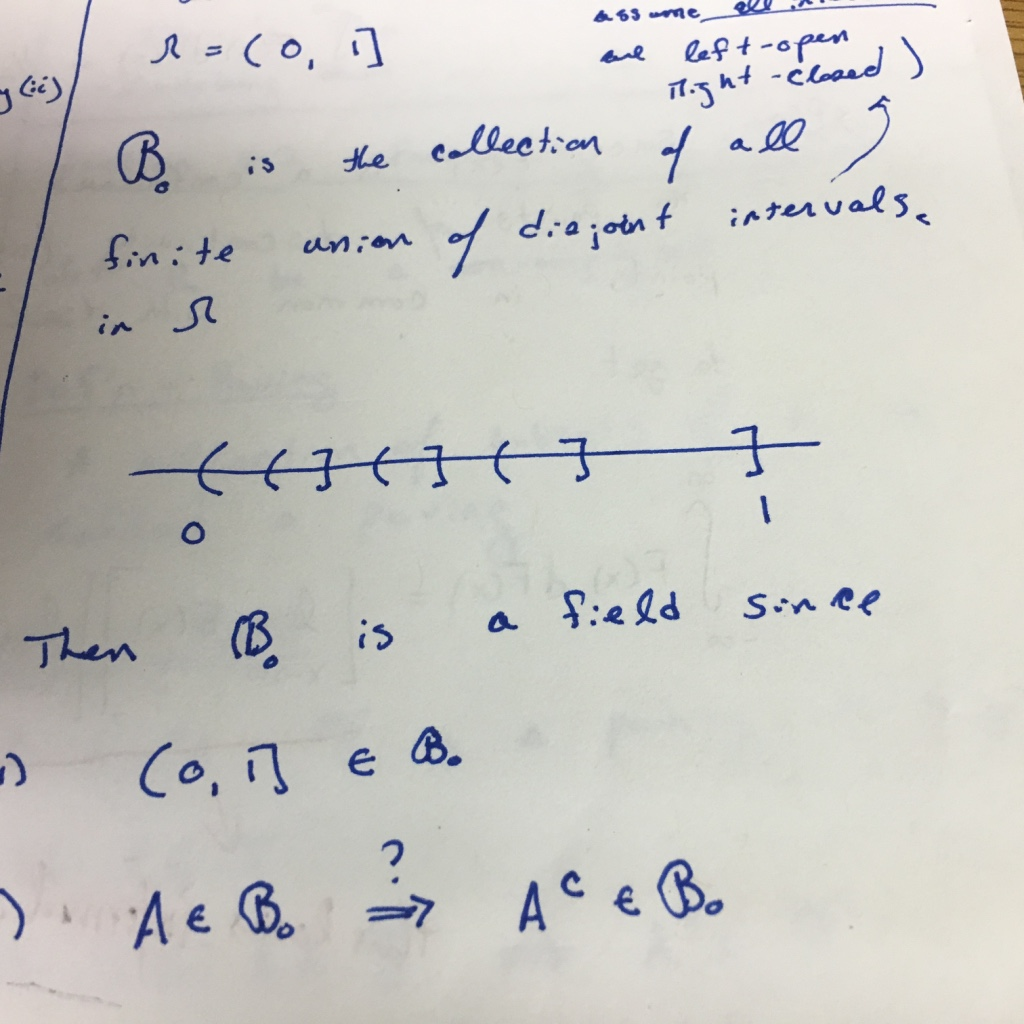
\includegraphics[scale=0.15]{notes1.jpg}
	\caption{Finite unioin of three disjoint intervals.}
	\end{figure}

	Then $\mathscr{B}_0$ is a field. 

	\begin{enumerate}[label = (\roman*)]
		\item (0, 1] $\in \mathscr{B}_0$
		\item $A \in \mathscr{B}_0 \Rightarrow A^c \in \mathscr{B}_0$ 
		\begin{figure}[h]
		\centering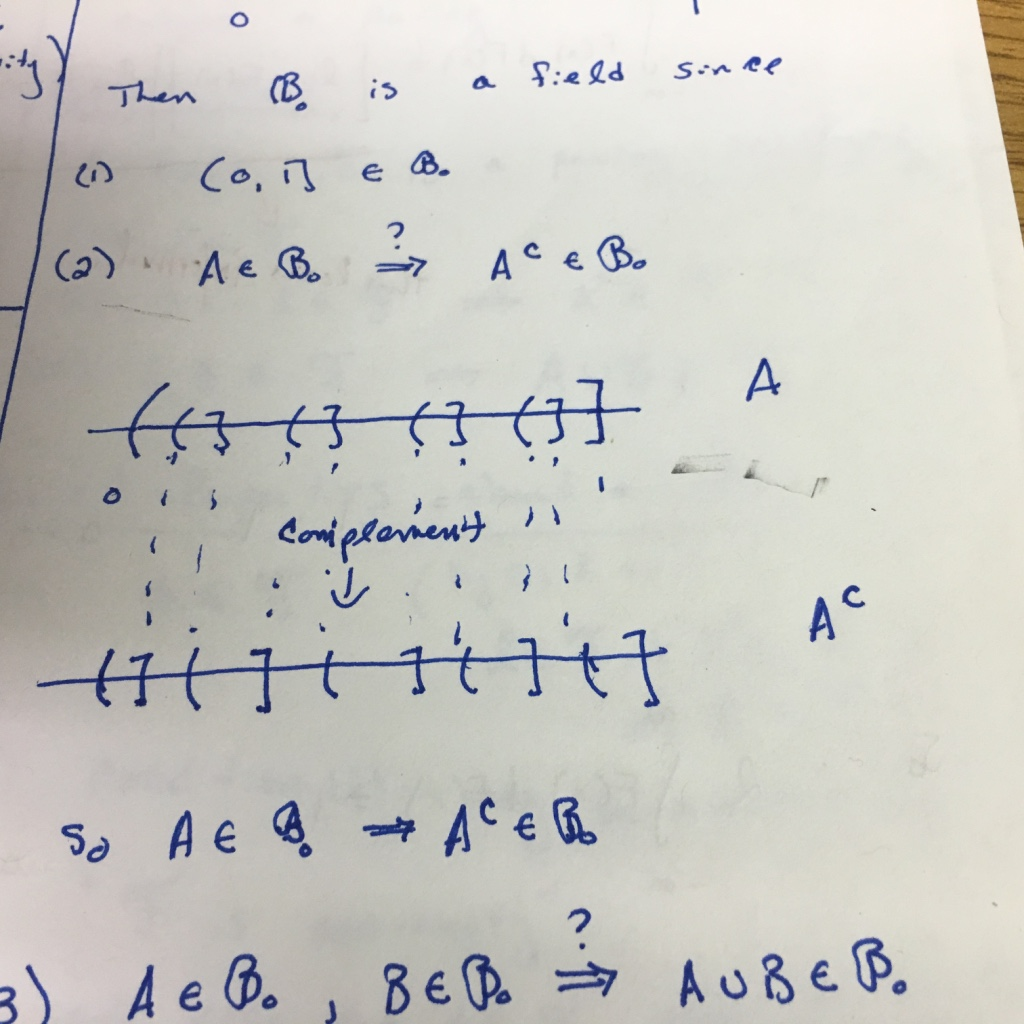
\includegraphics[scale=0.15]{notes2.jpg}
		\caption{A and complement of A.}
		\end{figure}

		\item $A \in \mathscr{B}_o, B \in \mathscr{B}_o \Rightarrow A \cup B \in \mathscr{B}_o$ 

		\begin{figure}[h]
		\centering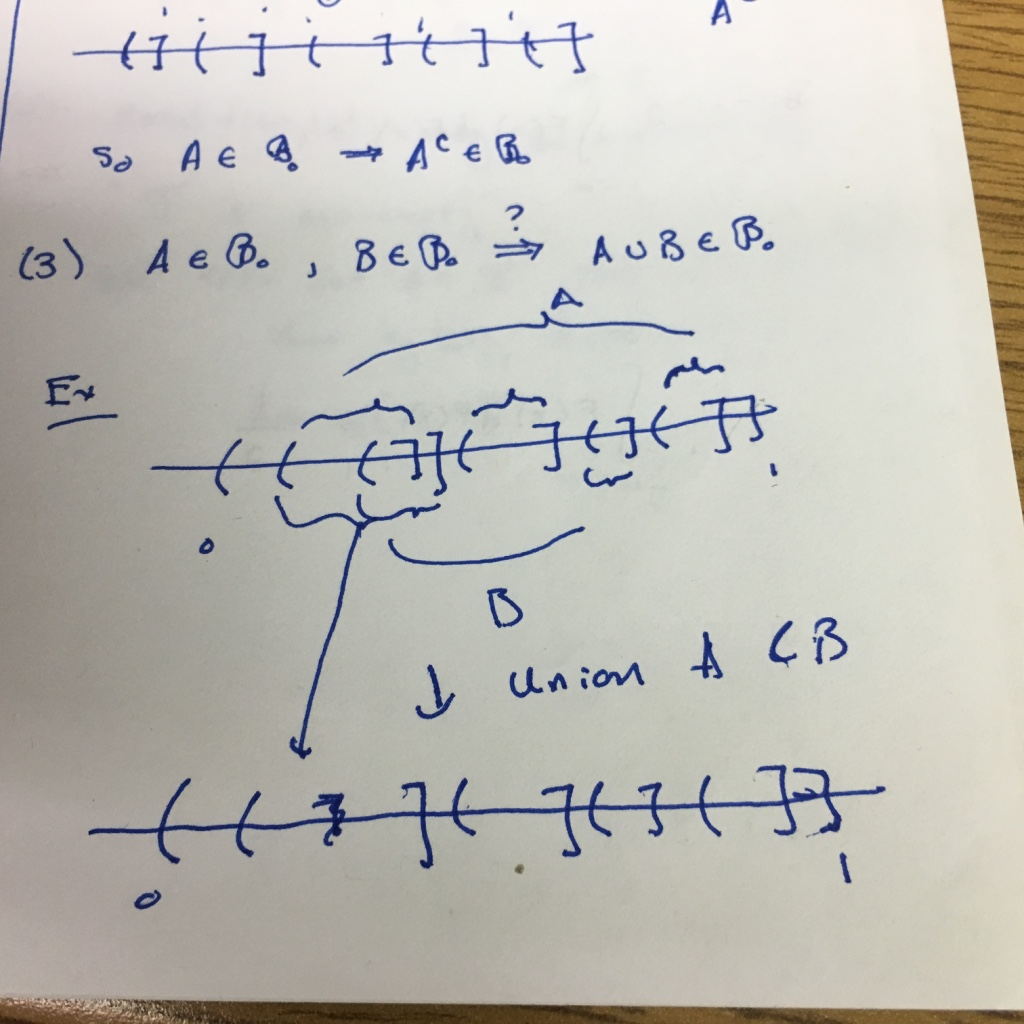
\includegraphics[scale=0.15]{notes3.jpg}
		\caption{Union of A and B is still in $\mathscr{B}_o$}
		\end{figure}

	\end{enumerate}


\end{example}


\textbf{Wednesday August 24}

$\mathscr{B}_0 = $ collection of finite unions of disjoin subintervals of (0, 1]. Is a field. \\
\\

\begin{definition}[Power Set]
	A $\sigma$-field is generated by a paving of power set. Let $\Omega$ be a set. The collection of all subsets of $\Omega$ is the power set written as $2^\Omega$.
\end{definition}

\begin{remark}
	Where does this notation come from?

Consider ths case where $\Omega$ is finite

$$\Omega = \{\omega_1, \dots, \omega_n \} $$

Total number of subsets of $\Omega$. 

$\emptyset, 1$ element sets, 2-element sets, $\dots$, n-element ests.

$$() + () + \dots + = (1+1)^n$$

$\#(\mathscr{F})  = 2^{\# \Omega}$, so it seems reasonable to denote $\mathscr{F} = 2^\Omega$. 

It is also easy to show that $2^\Omega$ is a $\sigma$-field. (The largest, even. The smallest: $\{\emptyset, \Omega\}$ which is also a $\sigma$-field.)

$$\{\emptyset, \Omega\} \subseteq \sigma\text{-field} \subseteq 2^\Omega$$ 
\end{remark}

It turns out we can extend notion of lenght from $\mathscr{B}_0$ to $\sigma$-field generated by $\mathscr{B}_o$. \\
\\
Now, let $\mathscr{A}$ be a nonempty paving of $\Omega$. We define 
$$\sigma(\mathscr{A}) = \cap \{\mathscr{B} \subseteq 2^\Omega: \mathscr{B}\text{ is a }\sigma\text{-field}, \mathscr{A} \subseteq \mathscr{B}\} $$

OR rather, the \textit{intersection} of all $\sigma$-fields that contains $\mathscr{A}$. \\
\\
Let 
$$\mathbb{F}(\mathscr{A}) = \{\mathscr{B} \subseteq 2^\Omega: \mathscr{B} \text{ is a } \sigma\text{-field, } \mathscr{B} \supseteq \mathscr{A} \}$$

Then, 
$$\sigma(\mathscr{A}) = \cap \mathscr{B}$$
$$\mathscr{B} \in \mathbb{F}(\mathscr{A}) $$

\textbf{Derived Facts}

$\mathbb{F}(\mathscr{A})$ is nonempty. For example, $2^\Omega$ is a $\sigma$-field and $2^\Omega \supseteq \mathscr{A}$. 

$\cap B$ is a $\sigma$-field. ($B \in \mathbb{F}(\mathscr{A})$)

\begin{remark}
	Get notes about notation/levels.
\end{remark}

\begin{proof} We will prove that indeed $\sigma(\mathscr{A})$ is a $\sigma$ -field. Recall that we have three conditions above for $\sigma$-field.\\
\\
	\begin{enumerate}[label = (\roman*)]
		\item $$\Omega \in \sigma(\mathscr{A})$$ 
			$$\Omega \in \cap_{B \in \mathbb{F}(\mathscr{A})} B $$
			Because: B is $\sigma$-field, $A \in B$, $\forall B \in \mathbb{F}(\mathscr{A})$.
		\item 
			% \begin{align*}
			% 	A \in \cap B &\Rightarrow A \in B \forall B \in\mathbb{F}(\mathscr{A})\\
			% 	&\Rightarrow A^C \in B , \forall B  \in \mathbb{F}(\mathscr{A})\\ 
			% 	&\Rightarrow A^C \in \cap_{B \in \mathbb{F}(\mathscr{A}) B\\
			% \end{align*}

		\item $A_1, \dots, \in \cap_{B \in \mathbb{F}(\mathscr{A})} B, \forall  B  \in \mathbb{F}(\mathscr{A})$

		$\Rightarrow \cup^\infty_{n =1} A_n \in B, \forall B \in \mathbb{F}(\mathscr{A})$

	\end{enumerate}

	So, $\sigma(\mathscr{A}$ is a $\sigma$-field, we call it the $\sigma$-field, generated by $\mathscr{B}_o$. We know how tot assign lenth to members of $\mathscr{B}_o$, we now show the assignment can be extended to $\sigma(\mathscr{B}_o)$ 


\end{proof}

\begin{example}
	 Let $\mathscr{I}$ be the collection of \textit{all} subintervals of (0,1].\\
	\\
	 Note that $\mathscr{I}$ is a smaller collection than $\mathscr{B}_0$ since $\mathscr{B}_0$ can have numerous different combinations of the sets. 

	 Let

	$$\mathscr{B} = \sigma(\mathscr{I})$$. 

	This is a Borel-$\sigma$-field. (a member of $\mathscr{B}$ in Borel set.)

	It turns out

	$$\sigma(\mathscr{I}) = \sigma(\mathscr{B}_o)  $$

This is because $\sigma(\mathscr{I})$ is a $\sigma$-field. 

So, 
	\begin{align*}
		\sigma(\mathscr{I}) &\supseteq \mathscr{B}_o\\
		\sigma(\mathscr{I}) &\supseteq \sigma(\mathscr{B}_o)
	\end{align*}

Also, 
\begin{align*}
		\mathscr{I} &\subseteq \mathscr{B}_o\\
		\sigma(\mathscr{I}) &\subseteq \sigma(\mathscr{B}_o)
	\end{align*} 

Thus, 
\begin{align*}
	\sigma(\mathscr{I}) &= \sigma(\mathscr{B}_o)
\end{align*}
\end{example}




\begin{definition}[Probability Measure]

Probablity measures on field. Suppose $\mathscr{F}$ is a field on a nonempy set $\Omega$. A probability measure is a function $P:\mathscr{F} \rightarrow \mathbb{R}$. 

\begin{enumerate}[label = (\roman*)]
	\item $0 \leq P(A) \leq 1, \forall A \in \mathscr{F}$
	\item $P(\emptyset) = 0$, $P(\Omega) = 1$
	\item If $A_1, \dots$ are disjoint emembers of $\mathscr{F}$ and $\cup A_n \in \mathscr{F}$ then we have countable additivity:

	$$P (\cup A_n) = \displaystyle\sum^\infty_{n=1} P(A_N) $$
\end{enumerate}

\begin{remark}
	Note that (iii) also implies finite additivity. Prove by adding infinite empty sets on end. 
\end{remark}

	
\end{definition}


If $\Omega$ is nonempty set. 
And $\mathscr{F}$ is a $\sigma$-field on $\Omega$.
And P is a probability measure on $\mathscr{F}$.

Then ($\Omega, \mathscr{F}, P$) is called a \textbf{probability space.}

And ($\Omega, \mathscr{F}$) is called a \textbf{measurable space.}


\begin{remark}
	If $A \subseteq B$, then $P(A) \leq P(B)$. This is because we may write B as

	$$B = A \cup (B\setminus A) $$
\end{remark}

\begin{remark}
	$$P(A) + P(B) = P(A\cup B) + P(A \cap B)$$


\end{remark}

\textbf{Friday August 26}
\\

Recall, 

Probability measure on a field, $\mathscr{F}_0$.

\begin{itemize}
	\item $P(A) + P(B) = P(A\cup B) + P(A \cap B)$

	% GET VINN DIAGRAM
	\begin{itemize}
		\item $P(A) = P(AB^C) + P(A B)$
		\item $P(B) = P(B A^C) + P(AB)$
		\item $P(A) + P(B) = P(AB^C) + P(BA^C) + 2P(AB)$
		\item $P(A \cup B) = P(AB^C) + P(BA^C) + P(AB)$ 
	\end{itemize}
	
	\item $P(A \cup B) = P(A) + P(B) - P(AB)$
		By induction, we can prove if $A_1, \dots A_n$,

		$$P(\displaystyle \cup^n_{k=1} A_k) = \displaystyle \sum^n_{k=1} P(A_k) - \displaystyle \sum_{i<j} P(A_iA_j) +
		\displaystyle \sum_{i<j<k} A_iA_j) + \dots + (-1)^{n+1} P(A_1, \dots, A_n)  $$

		Inclusion- Exclusion Formula

	\item If $A_1, \dots A_n \in \mathscr{F}$,

		$$B_1 = A_1 $$
		$$B_2 = A_2 \setminus A_1$$
		$$\vdots $$

		Then, 
		$$\displaystyle \cup^n_{k=1} A_k = \displaystyle \cup^n_{k=1} B_k $$

		but the $B_i$ are disjoint. Also $A_K \subseteq B_k \forall k=1, \dots, n$.

		$$ P(\displaystyle \cup^n_{k=1} A_k) = P(\displaystyle \cup^n_{k=1} B_k) = \displaystyle \sum^n_{k=1} B_k \leq \displaystyle \sum^n_{k=1} A_k$$

		Thus, $P(\displaystyle \cup^n_{k=1} A_k) \leq \displaystyle \sum^n_{k=1} A_k$. Finite subadditivity. 

\end{itemize}

Some conventions, 

If $A_1, \dots$ is a sequence of sets, we say $A_n \uparrow A$ if 

\begin{enumerate}
 	\item $A_1 \subseteq A_2 \subseteq \dots$
 	\item $\displaystyle \cup^\infty_{k=1} A_k = A$
 \end{enumerate} 
\vspace{5mm}
 If $A_1, \dots$ is a sequence of sets, we say $A_n \downarrow A$ if 

\begin{enumerate}
 	\item $A_1 \supseteq A_2 \supseteq \dots$
 	\item $\displaystyle \cap^\infty_{k=1} A_k = A$
 \end{enumerate} 

 \begin{theorem}
 	If $P$ is a probability measure on a field $\mathscr{F}$ Then, 

 	\begin{enumerate}
 		\item Continuity from below.

 		If $A_n \in \mathscr{F} \quad \forall n, A \in \mathscr{F}$
 		$$ A_n \uparrow A$$

 		then $$P(A_n) \uparrow P(A)$$

 		\item Continuity from above.

 		If $A_n \in \mathscr{F} \quad \forall n. A \in \mathscr{F}$  
 			$$A_n \downarrow A$$
 		 then $$P(A_n) \downarrow P(A)$$

 		\item Countable subadditivity.

 		If $A_n \in \mathscr{F} \quad \forall n. \displaystyle \cup^\infty_{k=1} A_k \in \mathscr{F}$ then 

 		$$P(\displaystyle \cup^\infty_{n=1} A_k) \leq \displaystyle \sum^\infty_{n=1} P(A_k)$$
 	\end{enumerate}
 \end{theorem}

 \begin{proof}

 \begin{enumerate}
 	\item If $A_1, \dots A_n \in \mathscr{F}$,

		$$B_1 = A_1 $$
		$$B_2 = A_2 \setminus A_1$$
		$$B_3 = A_3 \setminus A_2$$
		$$\vdots $$

		then, $B_1, \dots$ are disjoint. 

		$$\displaystyle \cup^\infty_{n=1} A_n = \displaystyle \cup^\infty_{n=1} B_n $$

		$\begin{aligned}
			P(A) &= P(\displaystyle \cup^\infty_{n=1} A_n) \\
		&= P(\displaystyle \cup^\infty_{n=1} B_n ) \\
		&= \displaystyle \sum^\infty_{n=1} P(B_n) \\
		&= \lim_{n \rightarrow \infty} \displaystyle \sum^\infty_{n=1} P(B_n)\\ 
		&= \lim_{n \rightarrow \infty} P(A_n)
		\end{aligned}
		$

	\item $A_n \downarrow A \Leftrightarrow A_n^C \uparrow A^C$

	But by (1), 

	$$P(A_n^C) \uparrow P(A^C)$$
	$$1 - P(A_n) \uparrow 1 - P(A)$$
	$$P(A_n) \downarrow P(A)$$


	\item By finite subadditivity, 

	$$ P(\displaystyle \cup^n{k=1} A_k) \leq \displaystyle \sum^n{k=1} P(A_k) \leq \displaystyle \sum^\infty_{n=1} P(A_n)$$

	But since, by (1), because

	$$\displaystyle \cup^n_{k=1} A_k \uparrow \displaystyle \cup^\infty_{n=1} A_n$$

	$$P(\displaystyle \cup^n_{k=1} A_k) \uparrow P(\displaystyle \cup^\infty_{n=1} A_n)$$

	So, 

	$$P(\displaystyle \cup^\infty_{n=1} A_n) \leq
		 \displaystyle \sum^\infty_{n=1} P(A_n)$$


 \end{enumerate}
\end{proof}

\begin{remark}
	$A \in \mathscr{F} =$ "A is F-set".
\end{remark}


\section{Extention of Probability Measure to a $\sigma$-field}\index{Exten. Prob Measure to $\sigma$-field}

Let $f$ be a function $f: D\rightarrow R$. 

Let $\tilde{D}$ be another set such that 

$$D \subseteq \tilde{D} $$

An extantion of $f$ onto  $\tilde{D}$ is 

$$\tilde{f}: \tilde{D} \rightarrow R $$

Such that $f(x) = \tilde{f}(x) \forall x \in D$

$\tilde{f}$ is an extention of $f$ on D. 

We say $f$ has unique extention, $\tilde{f}$ onto $\tilde{D}$ if 

\begin{enumerate}
	\item $\tilde{f}$ is an extension of $f$ to $\tilde{D}$.

	\item if $g$ is another extension of $f$ to $\tilde{D}$ then $\tilde{f} = g$ on $D$.
\end{enumerate}


\begin{theorem}
	A probability measure on a field has a unique extension on the $\sigma$-field generated by this field. 

		This means that if $\mathscr{F}_0$ is a field, and $P$ is a probability measure on $\mathscr{F}_0$, then there exists a probability measure, $Q$ on $\sigma(\mathscr{F})$ such that 
		$$Q(A) = P(A)\quad \forall A \in \mathscr{F}_0$$

		Moreover, if $\tilde{Q}$ is another probability measure on $\sigma(\mathscr{F}_0)$ such that $\tilde{Q} = P(A) \quad \forall A \in \mathscr{F}$ then $$\tilde{Q} = Q$$. 
\end{theorem}

	\begin{remark}
		The proof of this theorem will come after several definitions and lemmas. 
	\end{remark}

	\textbf{Outer Measure} $P^*: 2^\Omega \rightarrow \mathbb{R}$  

	For any $A \in 2^\Omega$ ($A \subseteq \Omega$)

	$$P^*(A) = \inf \{\displaystyle \sum_{n=1}^\infty P(A_n): A_1, A_2, \dots \text{is a sequence of } \mathscr{F}_0 \text{ sets, } A \subseteq \cup^\infty_{n=1} A_n\} $$

	$P^*$ is a measure out until $\mathscr{M}$, but it is only a function beyond that on $2^\Omega$.\\

\textbf{Inner Measure}

$P_*(A) = 1 - P^*(A)$ 

\vspace{5mm}

Define the paving $\mathscr{M}$ as followes
$$\mathscr{M} = \{ A \in 2^\Omega:
		E \in 2^\Omega,
		P^*(E) = P^*(E\cap A) + P^*(E \cap A^C) \}$$

	Idea: we came up with this $\mathscr{M}$ such that $P^*$ behaves as a measure. It will turn out to be that $\mathscr{M}$ is a $\sigma$-field that contains $\sigma(\mathscr{F}_0)$.\\

\textbf{Monday August 29}\\

$P^*$ satisfies the following probabilities:

\begin{enumerate}[label = (\roman*)]
	\item $P^*(\emptyset) = 0$
	\item $P^*(A) \geq 0 \quad \forall A \in 2^\Omega$
	\item $A \subseteq B \Rightarrow P^*(A) \subseteq P^*(B)$
	\item $P^*(\cup^\infty_{n=1} A_n) \leq \displaystyle \sum^\infty_{n=1} P^*(A_n))$
\end{enumerate}

\begin{proof}
	
	\begin{enumerate}[label = (\roman*)]
		\item Take $\{\emptyset, \emptyset, \dots \}$. 

		$$\emptyset \in \mathscr{F}_0, \quad \emptyset \cup^\infty_{n=1} \emptyset $$

		So, \\
		$$P^*(\emptyset) \leq \displaystyle \sum^\infty_{n=1} P(\emptyset) = 0$$

		Note,

		$$P(A) \geq 0 \quad \forall A$$

		So, 

		$$P^*(\emptyset) \geq \emptyset$$ 

		Thus,

		 $$P^*(\emptyset) = \emptyset$$
		\item  Already done as part of (i).

		\item  Let $A \subseteq B$

		$$P^*(A) = \inf\{\displaystyle \sum^\infty_{n=1} P(A_n), A_n \in \mathscr{F}_0, A \subseteq \cup A_n \} $$

		Now, if $B_1, \dots \in \mathscr{F}_0 \subseteq \cup B_n$

		Then, 
		$$A \subseteq B \subseteq \cup_n B_n $$

		If  $\{ \{B_n\}^\infty_{n=1}: B_n \in \mathscr{F}_0, B \subseteq \cup_n B_n \} \subseteq \{ \{A_n\}^\infty_{n=1}: A_n \in \mathscr{F}_0, A \subseteq \cup_n A_n \}$

		Or in short, Collection 1 $\subseteq$ Collection 2.\\

		So the inf of a larger set is smaller than (or equal to) the inf of a smaller set.\\
		
		So, 

		$P^*(A) = \inf\{\displaystyle \sum^\infty_{n=1} P(A_n), A_n \in  \text{ collection \#1}\} \leq P^*(B) = \inf\{\displaystyle \sum^\infty_{n=1} P(B_n), A_n \in  \text{ collection \#2}\} = P^*(B)$

		\item Want 

		$$P^*(\cup_n A_n) \leq \displaystyle\sum_n P^*(A_n) $$

		$P^*(A_n) = \inf \{\displaystyle \sum_{n=1}^\infty P(A_n): A_{nk} \in \mathscr{F}_0,  A \subseteq \cup_{k} A_{nk}\}$\\

		Let $\epsilon > 0$, by defnition of  there exists, 

		$$ \{B_n\}^\infty_{n=1}  $$ such that

		$$\displaystyle \sum^\infty_{k=1} P(B_{nk}) \leq P^*(A_n) + \frac{\epsilon}{2^n} $$

		So, 

		$$\cup_n A_n \subseteq \cup_{n,k} B_{nk} $$

		and,\\

		$\begin{aligned}
			P^*(\cup_n A_n) &\leq \displaystyle \sum_{n,k} P(B_{nk})\\ 
			&< \displaystyle \sum_n P^* (A_n) + \sum_n (\epsilon 2^{-n})\\
			P^*(\cup A_n) &< \sum_n P^* (A_n) + \epsilon \quad \forall \epsilon > 0
		\end{aligned}$

		Simply put, \\
		$ b$

		So, 

		$$P^*(\cup_n A_n) \leq \sum_n P^*(A_n) $$
 	\end{enumerate}
\end{proof}

By definition, $A \in \mathscr{M}$ if and only if $P^*(EA) + P^*(EA^C) = P^*(E)$. \\

We know that $P^*$ is subadditive. \\

So, by subadditivity we know, 

$$P^*(E) \leq P^*(AE) + P^*(A^C E) $$

Therefore, to show $A \in \mathscr{M}$ we only need to show 

$$P^*(E) \geq P^*(AE) + P^*(A^C E) $$


$\mathscr{M}$ is defined by $P^*$ and $P^*$ is defined using $\mathscr{F}_0$ so $\mathscr{M}$ is indireclty tied to $\mathscr{F}_0$.\\

\textbf{Lemma 1.} $\mathscr{M}$ is a field.

\begin{proof}


\begin{enumerate}[label = (\roman*)]
	\item $\Omega \in \mathscr{M}$\\

	$$\begin{aligned}
			A &= \Omega\\
			P^*(\emptyset) &= 0\\
			P^*(E) + P^*(\emptyset) &= P^*(E)
		\end{aligned}$$

	\item $A \in \mathscr{M} = A^C \in \mathscr{M}$\\

	$$\begin{aligned}
		P^*(E) &= P^*(EA) + P^*(A^C E)\\
		&= P^*(EA^C) + P^*(A E)\\
		&= P^*(EA^C) + P^*((A^C)^C E)
	\end{aligned}$$

	\item $A, B \in \mathscr{M} \rightarrow A \cap B \in \mathscr{M}$\\

	$B \in \mathscr{M} \Rightarrow P^*(E) = P^*(Eb) + P^*(B^C E) \quad \forall E$

	$A \in \mathscr{M} \Rightarrow P^*(BE) = P^*((BE)A) + P^*(A^C (BE))$

	$A \in \mathscr{M} \Rightarrow P^*(B^CE) = P^*((B^CE)A) + P^*(A^C (B^CE))$\\

	Hence, \\
	
	$$P^*(BE) + P^*(B^CE) = P^*((BE)A) + P^*(A^C (BE)) + P^*((B^CE)A) + P^*(A^C (B^CE))$$

	$$\begin{aligned}
		P^*(A^C (BE)) + P^*((B^CE)A) + P^*(A^C (B^CE)) &\geq P^*((A^C BE) \cup (AB^CE)\cup(A^CBE))\\
			&= P^*(E\cap[A^CB\cup  AB^C\cup A^CB^C])\\
			&= P^*(E \cap (AB)^C)
	\end{aligned} $$

	$$\begin{aligned}
		P^*(E) &= P^*(BE) + P^*(B^CE)\\
		&= P^*((BE)A) + (P^*(A^C (BE)) + P^*((B^CE)A) + P^*(A^C (B^CE)))\\
		&\geq P^*(ABE) + P^*(E(AB)^C)
	\end{aligned} $$
	
	 

	So, $A,B \in \mathscr{M}$
\end{enumerate}
\end{proof}

\textbf{Lemma 2.} If $A_1, A_2, \dots$ is a sequence of disjoint $\mathscr{M}$-sets then for each $E \subseteq \Omega$, 
$$P^*(E\cap(\cup_k A_k)) = \displaystyle \sum_k P^*(E \cap A_k) $$

\begin{proof}
	First, prove this statement for finite sequence. 

	$$A_1, \dots, A_n $$

	by mathematical induction. \\
	\\

	If $n=1$ this is 'trivial', 

	$$P^*(E\cap A_1) = P^*(E \cap A_1) $$

	If $n = 2$ we need to show, 

	$$ P^*(E  (A_1 \cup A_n)) = P^*(E A_1) + P^*(E A_2)$$

	Because $A_1 \in \mathscr{M}$, 

	$$P^*(E(A_1 \cup A_2)) = P^*(E(A_1 \cup A_2)) A_1 + P^*(E(A_1 \cup A_2)A_1^2)  $$

	$$E(A_1 \cup A_2) = E(A_1 A_2 \cup A_1 A_2 = EA_1$$

	$$E(A_1 \cup A_2) A_1^C = E(A_1 A_1^C \cup A_2 A_2^C)$$

	So, 

	$$P^*(E(A_1 \cup A_2)) = P^*(EA_1) + P^*(EA_2)$$

Suppose true for n = k. (induction hypothesis) \\
\\
Now we must show for n = k + 1.

$$P^* (E \cap (\cup_{n=1}^{k+1} A_n)) = P^*([E \cap (\cup_{n=1}^{k} A_n)] \cup A_{k+1}) $$

$ (\cup_{n=1}^{k} A_n), A_{k+1}$ are two disjoint sets. Using the n=2 case, 

$$ = \displaystyle \sum_{n=1}^k P^*(E \cap A_n) + P(E \cap A_{k+1}) = \displaystyle \sum_{n=1}^{k+1} P^*(E \cap A_n)  $$

So this is now shown to be true for $\{A_1, \dots, A_n \}$. Next, showtrue for $A_1, \dots in \mathscr{M}$ (disjoint).

Want: 

$$P^*(E \cap (\cup_{n=1}^\infty A_n)) = \displaystyle \sum_{n=1}^{\infty} P^*(E \cap A_n)  $$

Using countable subadditivity, 

$$ P^*(E \cap (\cup_{n=1}^\infty A_n)) = P^*(\displaystyle \cup_{n=1}^{\infty} E \cap A_n) \leq \displaystyle \sum_{n=1}^{\infty} P^*(E \cap A_n)$$

In the meantime, by the monotonicity of $P^*$

$$P^*(E \cap (\cup_{n=1}^\infty A_n)) \geq P^*(E \cap (\cup_{n=1}^m A_n)) =  \displaystyle \sum_{n=1}^{\infty} P^*(E \cap A_n)$$

So, 

$$P^*(E \cap (\cup_{n=1}^\infty A_n)) \geq \lim  \displaystyle \sum_{n=1}^{m} P^*(E \cap A_n)$$


(*), (**) gives us, 

$$P^*(E \cap (\cup_{n=1}^\infty A_n)) = \displaystyle \sum_{n=1}^{\infty} P^*(E \cap A_n)  $$

\end{proof}

\textbf{Wednesday August 31}

(finished proof)\\
\\

\textbf{Lemma 3.}
	
	\begin{enumerate}
		\item $\mathscr{M}$ is a $\sigma$-field
		\item $P^*$ restricted on $\mathscr{M}$ is countably additive. 
	\end{enumerate}

\begin{proof}
	First we show if\\

	\begin{enumerate}
		\item $\mathscr{M}$ is a fieldd
		\item $\mathscr{M}$ is closed under countable disjoint union.
	\end{enumerate}

then $\mathscr{M}$ is a $\sigma$-field.

Let's create disjoints sets, 

$A_n \in \mathscr{M}, n = 1, 2, \dots$
$B_1 = A_1$
$B_2 = A_2 A^C_1$
$\vdots$
$B_n = A_n A_1^C \dots A_{n-1}^C$

$B_1, \dots, B_n \in \mathscr{M}$ (disjoint)


$$\cup^\infty_{n=1} B_n = \cup^\infty_{n=1} A_n $$

But we know that $\cup^\infty_{n=1} B_n \in \mathscr{M}$ so $\cup^\infty_{n=1} A_n \in \mathscr{M}$ and thus $\mathscr{M}$ is a $\sigma$-field.

So it suffices to show that $\mathscr{M}$ is closed under disjoint countable unions.\\
\\
Let $A_1, A_2, \dots$ are disjoins $\mathscr{M}$-sets.\\ 
\\
Let $A = \cup^\infty_{n=1} A_n$.\\ 
\\
Let $F_n = \cup^n{k=1} A_k$.\\ 
\\
Then $F_n \in \mathscr{M}$.\\
\\
So, $\forall E \in 2^\Omega$, 

$$P^*(E) = P^*(E F_n) + P^*(E F_n^C) $$

\begin{align*}
	P^*(E F_n) &= P^*(E(\cup_{k=1}^n A_k))\\
		&= \displaystyle \sum^n_{k=1} P^*(E A_k)\\
P^*(E F_n^C) &\geq P^*(E A^C)  (F_n \subseteq A, F_n^C \supseteq A^C)\\
	\Rightarrow P^*(E) \geq \lim_{n \rightarrow \infty} P^*(E A_k) + P^*(E A^C)\\
		&= \displaystyle \sum^n_{k=1} P^*(E A_k) + P^*(E A^C)\\
		&= P^*(EA) + P^*(E A^C)
\end{align*}
 

\end{proof}

So $A \in \mathscr{M}$ and $\mathscr{M}$ is a $\sigma$-field. \\
\\

Now, let's show $P^*$ is countably additive.

Let $A_1, A_2, \dots$ be disjoint members of $\mathscr{M}$. Then $\forall E \in 2^\Omega$, 

$$P^*(E(\cup^\infty_{n=1} A_n)) = \displaystyle \sum^\infty_{n=1} P(E A_n) $$

Take $E = \Omega$. 

$$P^*(\cup^\infty_{n=1} A_n) = \displaystyle \sum^\infty_{n=1} P( A_n) $$


\textbf{Lemma 4.} $\mathscr{F}_0 \subseteq \mathscr{M}$

\begin{proof}
	Let $A \in \mathscr{F}$.\\
	\\

	Want:

	$$A \in \mathscr{M} $$
$$P^*(E) = P^*(EA) + P^*(E A^C) $$

By definition, there exists $E_n \in \mathscr{F}_0$ 
such that 

$$\displaystyle \sum^\infty_{n=1} P^*(E_n) \leq P^*(E) + \epsilon $$

$\begin{aligned}
	P^*(EA) &\leq P^*((\cup^\infty_{n=1} E_n)A) \text{ (monotonocity)}\\
		&= P^* (\cup^infty_{n=1} (E_n A))\\
		&\leq \displaystyle \sum^infty_{n=1}P^* ( (E_n A)) \text{ (countibly subadd)}\\
	P^*(E A^C) &\leq \displaystyle \sum^\infty_{n=1} P^*(E_n A^C)\\
	P^*(EA) + P^*(E A^C) &\leq 	\displaystyle \sum^\infty_{n=1} P^*(E_n A) + P^*(E_n A^C)\\
		&= \displaystyle \sum^\infty_{n=1} P^*(E_n)\\
	\text{Recall, } A, E_n \in \mathscr{F}_0\\
		&\leq P^*(E) + \epsilon\\
	P^*(EA) + P^*(E A^C) & \leq P^*(E) + \epsilon \quad \forall \epsilon\\
	\Rightarrow P^*(EA) + P^*(EA^C) &= P^*(E)\\
	\Rightarrow A \in \mathscr{M}\\
	\mathscr{F}_0 \in \mathscr{M}
\end{aligned}$
 
\end{proof}

\textbf{Lemma 5.}$$P^*(A) = P(A) \quad \forall A \in \mathscr{F}_0$$

\begin{proof}
	Let $A \in \mathscr{F}_0$. 

	Because,  $A, \emptyset, \emptyset, \dots, \in \mathscr{F}_0$. 

	$$A \subseteq A \cup \emptyset \cup \emptyset \dots $$

	$$P^*(A) \leq P(A) + P(\emptyset) + \dots $$

But, if 

$$A_n \in \mathscr{F}_0$$

$$A \subseteq \cup^\infty_{n=1} A_n $$

$$P^*(A) \leq \displaystyle \sum^\infty_{n=1} P(A_n)$$

$$\Rightarrow P^*(A) \leq \inf \displaystyle \sum^\infty_{n=1} P(A_n) $$

$$ = P^*(A)$$
\end{proof}

\textbf{Friday September 2}

\begin{remark}
	\textbf{5 Lemma Recap}

	\begin{tabular}{|p{0.9\linewidth}|}\hline % or any other width
\rule{0pt}{5ex}% for more vertical space
		
	\textbf{Lemma 1.} $\mathscr{M}$ is a field.

	\textbf{Lemma 2.} If $A_1, A_2, \dots$ is a sequence of disjoint $\mathscr{M}$-sets then for each $E \subseteq \Omega$, 
	$$P^*(E\cap(\cup_k A_k)) = \displaystyle \sum_k P^*(E \cap A_k) $$

	\textbf{Lemma 3.}
	
	\begin{enumerate}
		\item $\mathscr{M}$ is a $\sigma$-field
		\item $P^*$ restricted on $\mathscr{M}$ is countably additive. 
	\end{enumerate}
	
	\textbf{Lemma 4.} $$\mathscr{F}_0 \subseteq \mathscr{M}$$
	\textbf{Lemma 5.}$$P^*(A) = P(A) \quad \forall A \in \mathscr{F}_0$$
	\text{ }\\
	\\\hline
\end{tabular}
\end{remark}

Recall, Extension Theorem. That is, If $\mathscr{F}$ is a field and $P$ is a probability measure, then there exists a measure, $Q$ such that 

	$$Q(A) =  P(A) \quad \forall A \in \mathscr{F}_0$$

\begin{proof}
	By Lemma 5, \\
\\
	$P^*(\Omega) = P(\Omega) = 1$\\
	$P^*(\emptyset) = P(\emptyset) = 0$\\
	\\

	Outline of what we need to show:\\

	\begin{itemize}
		\item $ 0 \leq M(A) \leq 1$
		\item $M(\emptyset) = 0, \quad M(\Omega)=1$
		\item $M(\cup_n A_n) = \sum_n M(A_n)$
	\end{itemize}

	\vspace{5mm}

	Since $\forall A \in \mathscr{M}$, 

	$$\emptyset \subseteq A \subset \Omega $$

	then 

	$$ 0 \leq P^*(\emptyset) \leq P^*(A) \leq P^*(\Omega) \leq 1$$

	But, by Lemma 3, $P^*$ is contably additive on $\mathscr{M}$. So $P^*$ is probability measure on $\mathscr{M}$ (which is a $\sigma$-field, by Lemma 3).\\

	By Lemma 4, $\mathscr{F}_0 \subset \mathscr{M} \Rightarrow \sigma(\mathscr{F}_0 \subseteq \mathscr{M}$. So $P^*$ is also probabliity measure on $\sigma(\mathscr{F}_0).$\\

	Finally, by Lemma 5, again $P^*(A) = P(A)$, $P^*$ is an extention of $P$ form $\mathscr{F}_0$  to $\sigma(\mathscr{F}_0)$. \\
\end{proof}

\textit{Uniqueness of of the extention, $\pi-\lambda$ Theorem}\\

	Paving - $\{ \pi$-system and $\lambda$-system.$\}$ (?)\\

\begin{definition}[$\pi$-System]
	A class of subsets $\mathscr{P}$ of $\Omega$ is a $\pi$ system, if $$A, B \in \mathscr{P} \Rightarrow AB \in \mathscr{P}$$ 
\end{definition}
	
\begin{definition}[$\lambda$-System]
	A class $\mathscr{L}$ is a $\lambda$-system if 
		\begin{enumerate}[label = $\lambda$(\roman*)]
			\item $\Omega \in \mathscr{L}$ 
			\item $A \in \mathscr{L} \Rightarrow A^C \in \mathscr{L}$
			\item If $A_1, \dots \in \mathscr{L} $ are disjoint then $\cup^\infty_{n=1} A_n \in \mathscr{L}$
		\end{enumerate}
\end{definition}
	

	So, the only difference is "disjoint". Weaker than a $\sigma$-field (i.e. A $\sigma$-field is always a $\lambda$-system).

Note that $(\lambda_2)$ can be replace by $(\lambda_{2\prime})$ wherein

$$A, B \in \mathscr{F}, A \subseteq B, \Rightarrow B\setminus A \in \mathscr{L} $$

That is $\lambda_1, \lambda_2, \lambda_3 \Leftrightarrow \lambda_1, \lambda_{2\prime}, \lambda_3$\\

\textbf{Lemma 6.} A class of sets that is both $\pi$-systema and $\lambda$-system is a $\sigma$-field. 

\begin{proof}
	Suppose $\mathscr{F}$ is both $\pi$-system and $\lambda$-system.

By definition, 
\begin{enumerate}
			\item $\Omega \in \mathscr{F}$ 
			\item $A \in \mathscr{F} \Rightarrow A^C \in \mathscr{F}$
		\end{enumerate}

		Let $A_1, A_2, \dots$ be $\mathscr{F}$ sets. 

		Let's constructs disjoints sets, B

		\begin{align*}
			B_1 &= A_1\\
			B_2 &= A_1A_2^C\\
			\vdots
		\end{align*}

		Then $B_n$ are $\mathscr{F}$-sets (by $\lambda_{2\prime} - A_2^C = \Omega A)2^C \in \mathscr{F}$, by $\pi$-system, $A_1A_2^C \in \mathscr{F}$ ).\\

		By $\lambda_3$, 

		$$\cup_n^\infty B_n \in \mathscr{F} $$

		So, 

		$$\cup_n^\infty A_n \in \mathscr{F} $$

\end{proof}

\begin{theorem}[$\pi$-$\lambda$ Theorem]
	If $\mathscr{P}$ is in a $\pi$-system, $\mathscr{L}$ is in a $\lambda$-system, then 
	$$\mathscr{P} \subseteq \mathscr{L} \Rightarrow \sigma(\mathscr{P} \subseteq \mathscr{L}) $$
\end{theorem}

\begin{proof}
	Let $\lambda(\mathscr{P})$ be the intersection of all $\lambda$-system that contains $\mathscr{P}$. 

		$$ \lambda(\mathscr{P}) = \cap\{\mathscr{L}^\prime: \mathscr{L}^\prime \supseteq \mathscr{P}, \mathscr{L}^\prime \text{ is }\lambda\text{-set }\}$$

	$\lambda(\mathscr{P})$ is a $\lambda$-system.\\

	Goal: prove $\lambda(\mathscr{P})$ is a $\sigma$-field.
	So we want to show that $\lambda(\mathscr{P})$ is a $\pi$-system.

	\begin{enumerate}
		\item $\Omega \in \lambda(\mathscr{P})$?\\

			$$\Omega \in \mathscr{L}^\prime \quad \forall \mathscr{L}^\prime$$
			$$\Omega \in \lambda(\mathscr{P}) $$

		\item $A \in \lambda(\mathscr{P}) \Rightarrow A^C \in \lambda(\mathscr{P})$?\\

		$$A \in \lambda(\mathscr{P}) \Rightarrow A \in \cap\{\mathscr{L}^\prime: \mathscr{L}^\prime \supseteq \mathscr{P}, \mathscr{L}^\prime \text{ is }\lambda\text{-set }\} $$

		Then 

		$A \in \mathscr{L}^\prime$ for any $\mathscr{L}^\prime \supseteq \mathscr{P}, \mathscr{L}^\prime$ is $\lambda$-system. 

		$$\Rightarrow A^C \in \mathscr{L}^\prime $$

		$$\Rightarrow A^C \in  \cap\{\mathscr{L}^\prime: \mathscr{L}^\prime \supseteq \mathscr{P}, \mathscr{L}^\prime \text{ is }\lambda\text{-set }\} = \lambda(\mathscr{P})$$

		\item $A_1, A_2, \dots \in \lambda(\mathscr{P})$ are disjoint then $A_1, A_2, \dots \in \mathscr{L}^\prime \quad \forall \mathscr{L}^\prime$. 

		Then $\cup A_n \in \mathscr{L}^\prime (\mathscr{L}^\prime \lambda\text{-system})$

		So $\cup_n A_n \in \lambda(\mathscr{P})$. 

		We call $\lambda(\mathscr{P})$ the $\lambda$-system generated by $\mathscr{P}$.\\

		If we can say that $\lambda(\mathscr{P})$ is also a $\sigma$-field, then $\sigma(\mathscr{P}) \subseteq \lambda(\mathscr{P})$ because $\sigma(\mathscr{P})$ is smallest. So then, $\sigma(\mathscr{P}) \subseteq \mathscr{L}$ because $\lambda(\mathscr{P})$ is the small $\lambda$-system. 

		So it suffices to show that $\lambda(\mathscr{P})$ is a $\sigma$-field. But we know if $\lambda(\mathscr{P})$ is a system then $\lambda(\mathscr{P})$ is $\sigma$-field. So it suffices to show that $\lambda(\mathscr{P})$ is a $\pi$-system.  \\

		Construct again for any $A \in 2^\Omega \quad (A \subseteq \Omega)$, let

		$$\mathscr{L}_A = \{B: AB \in \lambda(\mathscr{P}) \}$$

		Claim: If $A \in \lambda(\mathscr{P})$ then $\mathscr{L}_A$ is $\lambda$-system.\\

		\begin{enumerate}
			\item $\Omega \in \mathscr{L}_A$? 
				$$A\Omega = A \in \mathscr{L}_A$$
			\item $(\lambda_2^\prime) : B_1, B_2 \in \mathscr{L}_A, B_1 \subseteq  B_2 \Rightarrow B_2B_1^C \in \mathscr{L}_A $?

			$$B_1 \in \mathscr{L}_A \Rightarrow AB_1 \in \lambda(\mathscr{P}) $$
			$$B_2 \in \mathscr{L}_A \Rightarrow AB_2 \in \lambda(\mathscr{P}) $$

			Since $AB_1 \subseteq AB_2$, $\lambda(\mathscr{P})$ is $\lambda$-system by ($\lambda_2^\prime$) for $\lambda(\mathscr{P})$

			% GET FROM PHOTO

			\item If $B_n$ is disjoint, $\mathscr{L}_A$-sets. 

			Want $\cup_n B_n$ because 

			$$B_n \in \mathscr{L}_A $$

			$$B_n A \in \lambda(\mathscr{P}) $$

			Because $B_n$ disjoint we know that $B_n A$ is also disjoint.

			Hence, 
			$$\cup_n(B_n A) \in \lambda(\mathscr{P})$$


		\end{enumerate}

	Claim: $\lambda(\mathscr{P})$ is $\pi$-sytem.

	\begin{enumerate}
		\item If $A \in \mathscr{P}$, then $\mathscr{P} \subseteq \mathscr{L}_A$

	Suppose $A \in \mathscr{P}$.

	Let $B \in \mathscr{P}$, then $AB \in \mathscr{P}$ ($\pi$-system), and $AB \in \lambda(\mathscr{P}) \Rightarrow B \in \mathscr{L}_A$

		\item If $A \in \mathscr{P}$ then $\lambda(\mathscr{P}) \subset \mathscr{L}_A$.

		\item If $A \in \lambda(\mathscr{P})$, then $\mathscr{P} \in \mathscr{L}_A$

		Suppose, $A \in \lambda(\mathscr{P})$ and let $B \in \mathscr{P}$. 

		By step 2,


			$\begin{aligned}
				A &\in \mathscr{L}_A\\
					&\Rightarrow AB \in \lambda(\mathscr{P})\\
					&\Rightarrow B \in \mathscr{L}_A	
			\end{aligned}$

		\item If $A \in \lambda(\mathscr{P})$, then $\lambda(\mathscr{P}) \subseteq \mathscr{L}_A$. This is because $\lambda(\mathscr{P})$ is the smallest $\lambda$-system, $\mathscr{L}_A$ is $\lambda$-system containing $\mathscr{P}$ (by step 3).\\

		Now show that $\lambda(\mathscr{P})$ is $\pi$-system.\\

		$A, B \in \lambda(\mathscr{P})$ because $A \in \lambda(\mathscr{P})$. We have that $\lambda(\mathscr{P}) \in \mathscr{L}_A$.\\

		So 
		$$B \in \mathscr{L}_A $$ 

		$$BA \in \lambda(\mathscr{P})$$

		Thus $\lambda(\mathscr{P})$ is $\pi$-system.
	\end{enumerate}
	\end{enumerate}
\end{proof}

\textbf{Wednesday September 7}

\begin{theorem}
	Suppose $P_1$ and $P_2$ are probability measures on $\sigma(\mathscr{P})$ where $\mathscr{P}$ is a $\pi$-system. If $P_1$ and $P_2$ agree on $\mathscr{P}$ (that is, $P_1(A) = P_2(A) \quad \forall A \in \mathscr{P}$) then they agree on $\sigma(\mathscr{P})$.
\end{theorem}

\begin{proof}
	Let $$\mathscr{L} = \{A \in \sigma(\mathscr{P}): P_1(A) = P_2 (A) \}$$

	Then $\mathscr{P} \subseteq \mathscr{L}$.\\

	It suffices to show that $\mathscr{L}$ is a $\lambda$-system (because if so, then $\sigma(\mathscr{P}) \subseteq \mathscr{L}$ - in fact, $\sigma(\mathscr{P}) = \mathscr{L}$). \\

	Show $\mathscr{L}$ is a $\lambda$-system.\\

	\begin{enumerate}
		\item $\Omega \in \mathscr{L}$?
			$$P_1(\Omega) = P_2(\Omega) = 1, \quad \Omega \in \mathscr{P}$$

		\item $A \in \mathscr{L}$

		$$ P_1(A) = P_2(A) \Rightarrow P_1(A^C) = P_2(A^C), \quad A^C \in \mathscr{L}$$

		\item $A \in \mathscr{L}$. $A_n$ disjoint. Want $\cup^\infty_{n=1} A_n \in \mathscr{L}$.

		Since

		$$A_n \in \mathscr{L} $$

		$$P_1(A_n) = P_2(A_n) \quad \forall n$$

		$$\displaystyle \sum^\infty_{n=1} P_1(A_n) = \displaystyle \sum^\infty_{n=1} P_2(A_n) $$

		$$P_1 \displaystyle \cup^\infty_{n=1} (A_n) = P_2 \displaystyle \cup^\infty_{n=1} (A_n) $$

		So, $\cup A_n \in \mathscr{L}$.


	\end{enumerate}
\end{proof}

So our extention of (and uniqueness of the extention of) $P$ on $\mathscr{F}_0$ to $\sigma(\mathscr{F}_0)$ is complete. We have shown the existance of $Q$ on $\mathscr{M}$. \\

Since $Q$ agrees with $P$ on $\mathscr{F}_0$ and $\mathscr{F}_0$ is a field, this implies that this is a $\pi$-system.

If you have another extention, say $\tilde{Q}$, then $\tilde{Q} = P$ on $\mathscr{F}_0$. That is, $\tilde{Q} = Q$ on $\mathscr{M}$, where $\mathscr{M}$ is a $\sigma$-field, which is a $\pi$
-system.\\

So by Theorem 1.3.3, 

$\tilde{Q} = Q$ on $\sigma(\mathscr{P})$. \\

So, Theorem 1.3.1, is completely proved. \\


Lemma 1 - Lemma 5 imply the extention.\\
$\pi-\lambda$ Theorem and Theorem 1.3.3 implies uniqueness. \\
This wraps up Theorem 1.3.1.\\



\textbf{Lebesque measure on (0,1]}

$$\Omega = (0,1]$$

Recall, $\mathscr{B}_0$ is the finite disjoint unions of intervals in (0,1] and that $\mathscr{B}_0$ is a field. \\

Let $\mathscr{B} = \sigma(\mathscr{B}_0)$.\\

For each $A \in \mathscr{B}_0$, 

$$A = \cup^n_{i=1} (a_i, b_i] $$

Let $\lambda(A) = \displaystyle \sum^n_{i=1} (b_i - a_i)$.\\

Question: Is $\lambda$ a probability measure on $\mathscr{B}_0$?

\begin{theorem}[Theorem 2.2 in Billingsly]

The set function $\lambda$ on $\mathscr{B}_0$ is a probability measure on $\mathscr{B}_0$.
	
\end{theorem}

\begin{proof}
	\begin{enumerate}
		\item $0 \leq \lambda(A) \leq 1$

		\item $$\lambda(\Omega) = \lambda((0,1]) = 1-0 = 1$$
		$$\lambda(\emptyset) = \lambda((0,0]) = 0$$


		\item This one requires Theorem 1.3 in Billingsly (proof omitted - calculus, blah).

		Theorem 1.3 - If I is an interval in (0,1] and $\{I_k: k=1, 2, \dots \}$ are disjoint intervas in (0,1] such that 

		$$I = \cup^\infty_{k=1} I_k$$

		then, 

		$$|I| = \displaystyle \sum^\infty_{k=1} |I_k| $$

		where |a| means length of interval a. 

		Since $\cup^{m_k}_{j=1} I_{kj} \in \mathscr{B}_0$ and $\cup^{m}_{i=1} I_{i} = \cup^\infty_{k=1}\cup^{m_k}_{j=1} I_{kj}$.\\

		Then 

		$$\lambda(A) \lambda(\cup^{m}_{i=1} I_{i}) = \displaystyle \sum^m_{i=1} |I_i| $$

		Since, $I_i \subset \cup^\infty_{k=1}\cup^{m_k}_{j=1} I_{kj}$, then 

		$$I_i = I_i(\cup^\infty_{k=1}\cup^{m_k}_{j=1} I_{kj}) = \cup^\infty_{k=1}\cup^{m_k}_{j=1} I_i I_{kj} $$

		By Theorem 1.3, 

		$$|I| = \displaystyle \sum^\infty_{k=1} \sum^{m_k}_{j=1} |I_i I_{jk}| $$

		$$\lambda(A) = \displaystyle \sum^m_{i=1} \sum^\infty_{k=1} \sum^{m_k}_{j=1} |I_i I_{jk}| = \displaystyle  \sum^\infty_{k=1} \sum^{m_k}_{j=1} \sum^m_{i=1}|I_i I_{jk}| $$

		Because $I_{jk} \subseteq \cup^m_{i=1} I_i$, we have that

		$$I_{kj} = \cup^m_{i=1} I_{kj} I_i $$

		Again by Theorem 1.3, (note that $I_{kj} I_i$ are disjoint intervals)

		$$|I_{kj} = \sum^m_{i=1}|I_i I_{jk}| $$

		So, $\lambda(A) = \sum^\infty_{k=1} \sum^{m_k}_{j=1} | I_{kj} | = \sum^\infty_{k=1} \lambda(A_k)$


	\end{enumerate}

	% FINISH PROOF

\end{proof}


\textbf{Friday September 9}\\

Finished above proof. \\

So $\lambda$ is a probability on $\mathscr{B}_0$. By Theorem 3.1, there exists a unique measure $\tau$ on $\sigma(\mathscr{B}_0) = \mathscr{B}$ such that 

		$$\tau(A) = \lambda(A) \quad \forall A \in \mathscr{B}_0 $$

$\tau$ is called \textbf{Lebesgue Measure} on (0,1]. We may still write it as $\lambda$.



% %------------------------------------------------



\section{Probabilities Concerning Sequences of Events}\index{Probabilities Concerning Sequences of Events}

\textit{Set Limit}\\

Let $(\Omega, \mathscr{F})$ be a measureable space (i.e. $\Omega$ is nonempty set and $\mathscr{F}$ is $\sigma$-field). \\

let $A_1, \dots \in \mathscr{F}$. We define 

$$\cap^\infty_{n=1} \cup^\infty_{k=n} A_k = \limsup_{n\rightarrow \infty} A_n $$

It is trivial to show that $\lim\sup_{n\rightarrow \infty} A_n \in \mathscr{F}$. 


$$ \cup^\infty_{n=1} \cap^\infty_{k=n} A_k = \liminf_{n\rightarrow \infty} A_n $$

We swapped intersection/union...what we are doing here?

$\omega$ (means outcome) $\in \Omega$

$$\omega \in \limsup_{n \rightarrow \infty} A_n \Leftrightarrow \omega \in \cap^\infty_{n=1} \cup^\infty_{k=n} A_k$$

$$\Leftrightarrow \omega \in \cup^\infty_{k=1} A_k \quad \forall n=1, 2, \dots $$

$$\Leftrightarrow \omega \in A_k \quad \text{ for some }k\geq n, \quad \forall n = 1, 2, \dots $$

$\Leftrightarrow \omega$ is in infinitely many k. 

Similarly, 

$$\omega \in \liminf_{n \rightarrow \infty} A_n \Leftrightarrow \omega \in \cup^\infty_{n=1} \cap^\infty_{k=n} A_k $$

$$ \Leftrightarrow \omega \in \cap^\infty_{k=1} A_k \quad \text{ for some } n=1, 2, \dots$$

$$\Leftrightarrow \omega \in A_k \quad \forall k\geq n, \quad \text{ for some } n $$

$$\Leftrightarrow \omega \in \text{ all but finitely many } A_k $$

So this is a much stronger requirement. Intuitively, if $\omega$ is in all but finitely many $A_k$, then it must be in infinitely many $A_k$ (i.e. $\liminf_{n \rightarrow \infty} A_n \subseteq \limsup_{n\rightarrow \infty} A_n$).\\ 


	For i > max(n,m), 

	\begin{align*}
		\cap_{k=m}^\infty A_k \subseteq A_i &\subseteq \cup_{k=n}^\infty A_k\\
		\Rightarrow \cup^\infty_{m=1}\cap^\infty_{k=m} A_k &\subseteq \cup_{k=n}^\infty A_k\\
		\Rightarrow \cup^\infty_{m=1}\cap^\infty_{k=m} A_k &\subseteq \cap^\infty_{n=1}\cup_{k=n} A_k\\
		\Rightarrow \liminf_{n \rightarrow \infty} A_n &\subseteq \limsup_{n \rightarrow \infty} A_n
	\end{align*}
	 
	 $$\cap^\infty_{k=n}A_k \uparrow \liminf_{n \rightarrow \infty} A_n $$
	 $$\cup^\infty_{k=n}A_k \downarrow \limsup_{n \rightarrow \infty} A_n $$

	 If $\liminf_{n \rightarrow \infty} A_n = \limsup_{n \rightarrow \infty} A_n$, then we say that the sequences $\{A_n\}$ has a limit, 

	 $$\lim_{n \rightarrow \infty} A_n = \liminf_{n \rightarrow \infty} A_n = \limsup_{n \rightarrow \infty} A_n $$

	 $$ \lim_{n \rightarrow \infty} A_n \in \mathscr{F}$$

	 Sometimes we write, 

	 $$ \limsup_{n \rightarrow \infty} A_n = [A_n \text{ i.o. }] $$

	 \begin{theorem}
	 	Suppose $(\Omega, \mathscr{F}, P)$ is a probability space and $A_n \in \mathscr{F} 	\quad n= 1, 2, \dots$.

	 	\begin{enumerate}[label = (\roman*)]
	 	 	\item $$\limsup_{n \rightarrow \infty} P( A_n) \leq P(\limsup_{n \rightarrow \infty} A_n) $$

	 	 	$$ \liminf_{n \rightarrow \infty} P( A_n) \geq P(\liminf_{n \rightarrow \infty} A_n)$$

	 	 	\item $A_n \rightarrow A (A = \lim_{n \rightarrow \infty} A_n)$, then we have continuity of probability of a set funciton: 

	 	 	$$\lim_{n \rightarrow \infty} P(A_n) = P (\lim_{n \rightarrow \infty} A_n) $$
	 	 \end{enumerate} 
	 \end{theorem}


\textbf{Monday September 12}

\begin{proof}
	\begin{enumerate}[label = (\roman*)]
		\item Let $B_n = \cap^\infty_{k=n} A_k$. 

			$$B_n \uparrow \liminf_{n } A_n $$

			By Theorem 2.1,  

			$$P(B_n) \uparrow P(\liminf_{n } A_n) $$
			So, 

			$$P(B_n) \leq P(\liminf_{n } A_n) \quad \forall n $$

			$$\lim_{n \rightarrow \infty} P(B_n)  = P(\liminf_{n} A_n)$$

			$$P(A_n) \geq P(B_n) \rightarrow P(\liminf_n A_n) $$

			$$\liminf_n P(A_n) \geq P(\liminf_{n} A_n)$$

			Similarly, 

			Let $C_n = \cup^\infty_{k=n} A_k$. 

			Then, 

			$$ C_n \downarrow \cup^\infty_{k=n} A_k$$

			$$P(A_n) \leq P(C_n) \rightarrow P(\limsup_{n } A_n) $$

			$$ \limsup_{n }P( A_n) \leq  P(\limsup_{n } A_n)$$

			\item If $A_n$ has a limit (i.e. $\limsup_n A_n = \limsup_n A_n = \lim A$) then,

			$$\liminf_n P(A_n) \geq P(\liminf_n A_n) = P(\limsup_n A_n) \geq \limsup_n P(A_n) $$

			So, $\liminf_n P(A_n) = \limsup_n P(A_n)$, thus

			$$\lim_n P(A_n) = P(\lim_n A_n) $$

	\end{enumerate}
\end{proof}


Independent Events\\

$(\Omega, \mathscr{F}, P)$\\

Let $A, B \in \mathscr{F}$. They are independent if and only iff: 

$$P(AB) = P(A)P(B) $$
$$A \indep B  $$

$A_1, \dots A_n$ are independent if and only if for any $\{k_1, \dots, k_j \} \subseteq \{1, \dots, n\}$, 

$$P(A_{k_1} \dots A_{k_j}) = P(A_{k_1}) \dots P(A_{k_i}) $$

In this case we write: $A_1 \indep \dots \indep A_n$.\\


Now let, $\mathscr{A}_1, \dots, \mathscr{A}_n$ be pavings in $\mathscr{F}$ (i.e. $\mathscr{A}_k \subseteq \mathscr{F}$). \\

We say $\mathscr{A}_1, \dots, \mathscr{A}_n$ are independent if and only if for any $A_1 \in \mathscr{A}_1, \dots, A_n \in \mathscr{A}_n$ we have 

$$A_1 \indep \dots \indep A_n $$. 

In this case we write: $\mathscr{A}_1 \indep \dots \indep \mathscr{A}_n$.

\begin{theorem}
	Suppose for $(\Omega, \mathscr{F}, P)$ is a probability space if, 

	$$\mathscr{A}_1 \subseteq \mathscr{F} \dots \mathscr{A}_n \subseteq \mathscr{F}$$

	are $\pi$-systems. Then,

	$$\mathscr{A}_1 \indep \dots \indep \mathscr{A}_n  \Rightarrow \sigma(\mathscr{A}_1) \indep \dots \indep \sigma(\mathscr{A}_n)$$
\end{theorem}

\begin{proof}
	Let $\mathscr{B}_i = \mathscr{A}_i \cup \{\Omega\}$. 

	It is easy to show (in homework)

	\begin{enumerate}
		\item $\mathscr{B}_i$ is still a $\pi$-system
		\item $\mathscr{B}_i$ are still independent
		$$\mathscr{B}_1 \indep \dots \indep \mathscr{B}_n $$
	\end{enumerate}

	For $B_2 \in \mathscr{B}_n, \dots, B_n \in \mathscr{B}_n$ define, 

	$$\mathscr{L}(B_2, \dots, B_n) = \{B \in \mathscr{F}: B \indep B_2 \indep \dots \indep B_N \}$$


	\begin{enumerate}
		\item First we show $\mathscr{L}(B_2, \dots, B_n)$ is $\lambda$-system. 

	$$\Omega \in \mathscr{L}(B_2, \dots, B_n) $$
	$$\Omega \indep B_1 \indep \dots \indep B_n $$

	This is true because $P(\Omega B_2 \dots B_n) = P(B_2 \dots B_n) = P(B_2)\dots P(B_n) = P(\Omega)P(B_2)\dots P(B_n)$
		\item Now $A \in \mathscr{L}(B_2, \dots, B_n) \Rightarrow A^C \in \mathscr{L}(B_2, \dots, B_n)$

		$\begin{aligned}
				A \&in \mathscr{L}(B_2, \dots, B_n)\\
				&\Rightarrow A \indep B_2 \indep \dots \indep B_n	\\
				&\Rightarrow P(A B_2 \dots B_n) = P(A)P(B_2)\dots P(B_n)\\
				&\Rightarrow P(A^C B_2 \dots B_n)\\
				&\quad P(B_2 \dots B_n) \setminus A B_2 \dots B_n)\\
				&\quad P(B_2 \dots B_n) - P(A B_2 \dots B_n)\\
				&\quad P(B_2)\dots P(B_n) - P(A)P(B_2)\dots P(B_n)\\
				&\quad (1-P(A))P(B_2) \dots P(B_n) \ P(A^C)P(B_2)\dots P(B_n)\\
		\end{aligned}$

		Then we run this through all subadditives of $A, B_2, \dots, B_n$. 

		$A^C \indep B_2 \indep \dots \indep B_n$

		\item If $C_1, C_2, \dots, \in \mathscr{L}(B_2, \dots, B_n)$ they are disjoint. Want to show 
		$$\cup^infty_{m=1}C_m \in \mathscr{L}(B_2, \dots, B_n) $$

		$\begin{aligned}
			C_m \in \mathscr{L}(B_2, \dots, B_n)\\
			&\Rightarrow C_m \indep \dots \indep B_n\\
			&\Rightarrow P(C_m B_2 \dots B_n) = P(C_m)\dots P(B_n) \quad \forall m = 1, 2 \dots\\
			\displaystyle \sum^\infty_{m=1} P(C_m B_2 \dots B_n) &= (\displaystyle \sum^\infty_{m=1} P(C_m) )P(B_2)\dots P(B_n)
		\end{aligned}$

		But $\{C_m, B_2, \dots, B_n, m = 1, 2 \dots \}$

		% GET MORE OF PROOF

		
	\end{enumerate}
 So $\cup_m C_m \in \mathscr{L}(B_2, \dots, B_n)$. 

		And $\mathscr{L}(B_2, \dots, B_n)$. 

		Also, $ B_1 \in \mathscr{L}(B_2, \dots, B_n) \quad \forall B_1 \in \mathscr{B}_1$ therefore by definition, 

		$$\mathscr{B}_1 \subseteq \mathscr{L}(B_2, \dots, B_n) $$

So, $ \sigma(\mathscr{B}_1) \subseteq \mathscr{L}(B_2, \dots, B_n)$ and we have our $\lambda-\pi$-theorem.

This means that for all $B_1 \in \sigma(\mathscr{B}_1)$

$$B_1 \indep B_2 \indep \dots \indep B_n $$

Recall that $B_i $ are arbitrary members of,

$$\sigma(\mathscr{B}_1) \indep B_2 \indep \dots \indep B_n \Leftrightarrow \mathscr{B}_2 \indep \sigma(\mathscr{B}_1) \indep \dots \indep \mathscr{B}_n$$

Run the previous argument repeatedly. 

So

$$ \sigma(\mathscr{B}_1) \indep \sigma(\mathscr{B}_2) \indep \dots \indep \sigma(\mathscr{B}_n)$$ 

\end{proof}


\begin{example}
	Let $\mathscr{I}$ be the collection of all intervals, then its $\pi$-system. When we want to check $X \indep Y$, we only need to check

	$$P(X \in \text{interval}, Y \in \text{interval}) = P(X \in \text{interval})P(Y \in \text{interval}) $$
\end{example}

\textbf{Wednesday September 14}\\

\textbf{Indepencence of Infinite Classes}\\

Let $\{\mathscr{A}_\theta: \theta \in \Theta \}$ where $\theta$ is any infinite set (need not be countable) if and only if any (infinite) $\{A_\theta: \theta \in \Theta \}$ where $A_\theta \in \mathscr{A}_\theta$ are independent. \\

We alraedy define independence of $\{A_\theta: \theta \in \Theta \}$; that is for an infinite collection of sets is independent if and only if any finite subcollection $\{ A_{\theta_1}, \dots A_{\theta_n} \}$ is independent.\\

With this device, we may make claims such as

$$\{X_t: t \in (0,1] \} $$ 

are independent. Useful for stochastic process, functional data analysis.\\

It follows trivially, $\{\mathscr{A}_\theta: \theta \in \Theta \}$ are independent if and only if any finite collection, say $\{\mathscr{A}_{\theta_1}, \dots, \mathscr{A}_{\theta_n} \}$ are independent. 

\begin{corollary}[To Theorem 4.2]
	If $(\Omega, \mathscr{F}, P), \mathscr{A}_\theta \subset \mathscr{F}$,  $\{\mathscr{A}_\theta: \theta \in \Theta \}$ is independent and each $\mathscr{A}_\theta$ is a $\pi$-system, then

	$$\{ \sigma(\mathscr{A}_\theta): \theta \in \Theta \}$$

	are independent. 
\end{corollary}

\begin{proof}
	\begin{align*}
		\{\mathscr{A}_\theta: \theta \in \Theta \} \indep &\Leftrightarrow \{\mathscr{A}_{\theta_1}, \dots, \mathscr{A}_{\theta_n} \} \indep \\
		&\Leftrightarrow \{ \sigma(\mathscr{A}_{\theta_1}), \dots, \sigma(\mathscr{A}_{\theta_n}) \} \indep
	\end{align*}

\end{proof}

\begin{corollary}
	Suppose we have an array of sets, 

	$\begin{matrix}
			A_{11} & A_{12} & \dots & \dots\\
			A_{21} & A_{22} & \dots & \dots\\ 
			\vdots & \vdots & &\\
  			\vdots & \vdots & &\\
		\end{matrix} = \{A_{ij}: i,j = 1, \dots \} \subset \mathscr{F}$

		and this array is independent. \\

		And let $\mathscr{F}_i = \sigma(A_{i1}, A_{i2}, \dots)$.\\

		Then $\mathscr{F}_1 \indep \mathscr{F}_2$
\end{corollary}

\begin{proof}
	Let $\mathscr{A}_i$ be the class of all the finite intersections of 

	$$A_{i1}, A_{i2}, \dots$$

	then $\mathscr{A}_i$ is a $\pi$-system. \\

	So, 

	$$\sigma(\mathscr{A}_i) = \mathscr{F}_i $$

	because $\{A_{i1}, A_{i2}, \dots \}$ are contained in $\mathscr{A}_i$ which implies $\mathscr{F}_i \subset \sigma(\mathscr{A}_i)$ and also $\mathscr{A}_i \subset \mathscr{F}_i \Rightarrow \sigma(\mathscr{A}_i \leq \mathscr{F}_i$.

	By Corollary 1, it suffices to show that $\mathscr{A}_1, \mathscr{A}_2, \dots$ are independent. Further, it suffices to show that any finite subcollection is independent.\\

	Let $\{i_1, \dots, i_n \} \subseteq \{1, 2, \dots \}$. We want to show that $\mathscr{A}_{i_1}\indep \dots \indep \mathscr{A}_{i_n}$. This would be implied by the following

	$$\forall C_{i_1} \in \mathscr{A}_{i_1}, \dots, C_{i_n} \in \mathscr{A}_{i_n} $$

	$$C_{i_1} \indep \dots \indep C_{i_n}$$

	Because, and watch out with this notation here, for

			$$C_{i_\alpha} \in \mathscr{A}_{i_\alpha} $$

		there exists

		$${A}_{i_\alpha j_1}, {A}_{i_\alpha j_2}, \dots, {A}_{i_\alpha j_{m_\alpha}} $$

		such that

		$$C_{i_\alpha} = {A}_{i_\alpha j_1}, {A}_{i_\alpha j_2}, \dots, {A}_{i_\alpha j_{m_\alpha}} $$

		We have

		$$ P(\cap^n_{\alpha = 1} C_{i_\alpha}) = P(\cap^n_{\alpha = 1} \cup^{m_\alpha}_{\beta = 1} A_{i_\alpha j_\beta})$$

		because 

		$$\{A_{i_\alpha j_\beta}: \alpha, = 1, 2, \dots, n , \beta = 1, 2, \dots m_\alpha\} \subseteq \{ A_{ij}: i, j = 1, 2, \dots\}$$

		\begin{align*}
			P(\cap^n_{\alpha = 1} \cup^{m_\alpha}_{\beta = 1} P(A_{i_\alpha j_\beta}) &= \displaystyle \prod^n_{\alpha = 1} \prod^{m_\alpha}_{\beta = 1} P(A_{i_\alpha j_\beta})\\
			&= \displaystyle \prod^n_{\alpha = 1} P(C_{i_\alpha})
		\end{align*}
		% FINISH PROOF
\end{proof}


\textbf{Borel-Cantelli Lemmas (that are actually Theorems)}


\begin{theorem}[BC1]	
	For $(\Omega, \mathscr{F}, P)$ probability space, 

	$$A_n \in \mathscr{F}, \quad n= 1, 2, \dots$$

	If $\displaystyle \sum^\infty_{n=1} P(A_n) < + \infty$ then

	$$P(\limsup_{n \rightarrow \infty} A_n) = 0 $$
\end{theorem}	

\begin{proof}
	$\limsup_{n \rightarrow \infty} A_n = \cap^\infty_{n=1} \cup^\infty_{k=n} A_k \subset \cup^\infty_{k=n} P(A_k) \quad \forall n$

	So, 

	$$P(\limsup_{n \rightarrow \infty} A_n) \leq P( \cup^\infty_{k=n} P(A_k)) \leq \sum^\infty_{k=1} P(A_k)$$

	% FINISH
\end{proof}

\begin{theorem}[BC2]
	If $\{A_n\}$ are independent and $\displaystyle \sum^\infty_{n=1} P(A_n) = \infty$, then

	$$P(\limsup_n A_n) = 1 $$
\end{theorem}

\begin{proof}
	$P(\limsup_n A_n) = 1$

	$$\Leftrightarrow P(\bigcap^\infty_{n=1} \cup^\infty_{k=n} A_k) = 1 $$

	$$\Leftrightarrow P(\cup^\infty_{n=1} \cap^\infty_{k=n} A^C_k) = 0 \quad (*)$$

	because, 

	$$\Leftrightarrow P(\cup^\infty_{n=1} \cap^\infty_{k=n} A^C_k) \leq \displaystyle \sum^\infty_{k=n} P(\cap^\infty_{k=n} A_k^C )  $$

	$$\Leftarrow P(\cap^\infty_{k=n} A_k^C ) = 0 \quad \forall n = 1, 2, \dots $$

	but we need to prove this to imply (*). 

	Shit, calculus. 

	$$1 - x \leq e^{-1} \quad \forall x \in \mathbb{R} $$


	For any $j = 1, 2, \dots$, 
	\begin{align*}
		P\left( \bigcap^{n+j}_{k=n} A_k^C \right) &= \prod^{n+j}_{k=n} (1 - P(A_k))\\
			&\leq \prod^{n+j}_{k=n} e^{-P(A_k)}\\
			&= e^{- \sum^{n+j}_{k=n} P(A_k)}\\
	\end{align*}

	Now,  $\sum^{\infty}_{k=1} P(A_k) = \infty$ and also

	$$ \sum^{\infty}_{k=n} P(A_k) \quad \forall n $$

	So, 

	$$\lim \sum^{n+j}_{k=n} P(A_k) \rightarrow \infty \quad \forall n$$

	$$\lim_{j \rightarrow \infty} P\left(\bigcap^{n+j}_{k=n} A_k^C \right) = 0 $$

	Because, 

	$$\bigcap^{n+j}_{k=n} A_k^C \downarrow \bigcap^{infty}_{k=n} A_k^C \quad j \rightarrow \infty $$

	By continuity of probability, 

	$$ P\left(\bigcap^{n+j}_{k=n} A_k^C \right) \downarrow P\left(\bigcap^{infty}_{k=n} A_k^C \right)\quad j \rightarrow \infty$$

	So, 

	$$P\left(\bigcap^{infty}_{k=n} A_k^C \right) = 0 $$

\end{proof}

\textbf{Friday September 16}\\

finished proof. \\

BC1 and BC@ say that  $P \left(\limsup_n A_n \right)$ is either 0 or 1.\\

This is a special case of a general phonemonon, the 0-1 Law.

Take $\sigma$-field, $(\Omega, \mathscr{F}, P)$, 

$$A_1, \dots \in \mathscr{F} $$

For each n, 

$$\sigma(A_n, A_{n+1}, dots) $$

We have another $\sigma$-field called "tail of $\sigma$-field",

$$\mathscr{T} =  \bigcap^\infty_{n=1} \sigma(\mathscr{A}_n, \mathscr{A}_{n+1}, \dots) $$

\begin{example}[4.18 in Billingsly]
	$\limsup A_n \in \mathscr{T}$?

		$$\bigcap^\infty_n=1 \bigcup^infty_{n=k}  A_k  $$

		$$ A_n, A_{n+1}, \dots \in \sigma(\mathscr{A}_n, \mathscr{A}_{n+1}, \dots) \Rightarrow \bigcup^\infty_{k=n} A_k \in \sigma(\mathscr{A}_n, \mathscr{A}_{n+1}, \dots)$$

		$$\bigcap^\infty_n=1 \bigcup^\infty_{n=k}  A_k \in \bigcap^\infty_{n=1} \sigma(\mathscr{A}_n, \mathscr{A}_{n+1}, \dots) $$

	$\begin{aligned}
		\liminf A_n &= \left[ (\bigcup^\infty_n=1 \bigcap^\infty_{n=k}  A_k )^C \right]^C\\
			&= \left[ \bigcup^\infty_n=1 \bigcap^\infty_{n=k}  A_k^C \right]^C\\
			&= \left[\limsup_n A_k^C \right]^C \in \mathscr{T}
	\end{aligned}
	$


\end{example}



\begin{theorem}
	If $A_1, A_2, \dots$ are independent, then for each $A \in \mathscr{T}$ we have $P(A) = $ 0 or 1.
\end{theorem}

\begin{proof}
	By Corollary 2, 

	$\begin{matrix}
		\sigma(A_1)\\
		\sigma(A_2)\\
		\vdots\\
		\vdots\\
		\sigma(A_{n-1})\\
		\sigma(A_n, A_{n+1}, \dots)\\
	\end{matrix}$

	$$\sigma(A_1) \indep \dots \indep \sigma(A_n, A_{n+1}, \dots)$$

	Let $A \in \mathscr{T}$, then,

	$$A \in \sigma(A_n, A_{n+1}, \dots) \quad \forall n$$

	So, $A_1, \dots, A_{n-1}, A$ are independent. By taking nlarge enough, this implies that any  finite subcollectoin of $A, A_1, A_2, \dots$ is also independent. \\

	This implies that the sequence $\{ A, A_1, A_2, \dots\}$ are independent. \\

	But $A \in \sigma(A_1, A_2, \dots)$ so, 

	$$A \indep A$$

	$$ P(AA) = P(A)P(A) = P(A)^2 $$

	So $P(A)$ must be zero or 1! 

\end{proof}

\begin{remark}
	We are now skipping a few sections (5 -9) in Billingsly. These are about special random variables, random walks, etc...
\end{remark}





\section{General Measure on a Field}\index{General Measure on a Field}





\textbf{Borel Sets in $\mathbb{R}^k$}\\

Two jumps, from $(0,1] \rightarrow \mathbb{R} \rightarrow \mathbb{R}^k$.

$\mathscr{B} \text{ on } (0,1]$ is a $\sigma$-field generated by $\mathscr{J} = $ collection of all intervals in (0,1].

	$$\sigma(\mathscr{I}) = \mathscr{B} \text{ on } (0,1]$$

When we work with $\mathbb{R}$, 

$$\mathscr{I}^\prime = \text{collection of all intervals in } \mathbb{R}, (a,b) $$

$$\sigma(\mathscr{I}^\prime) = \mathscr{R}^\prime \quad \text{linear Borel }\sigma\text{-field} $$


$\mathscr{I}^k $ is the collection of all rectangles in $\mathbb{R}^k$.

$$ \mathscr{I}^k = \{(a_1, b_1]x \dots x(a_k, b_k]: a_1, b_1, \dots, a_k, b_k \in \mathbb{R} \}$$

$$\sigma(\mathscr{I}^k) = \mathscr{R}^k \quad \text{Borel } \sigma\text{-field in } \mathbb{R}^k$$

\textit{Properties of $\mathbb{R}^k$}\\

Any open set are in $\mathscr{R}^k$.\\

Let $\mathbb{Q}$ be the set of all rational numbers. This is countable and dense subset of $\mathbb{R}$. \\

\begin{definition}[Dense]
	Look up definition!
\end{definition}

Class of rational rectangles: 

$$ \mathscr{I}^k_\mathbb{Q} = \{(a_1, b_1]x \dots x(a_k, b_k]: a_1, b_1, \dots, a_k, b_k \in \mathbb{Q} \}$$

Let G be an open set in $\mathbb{R}^k$ and $y \in G$, then there exists
 
$$ A_y \in  \mathscr{I}^k_Q $$

such that

$$y \in A_y \subset G $$

because $\mathbb{Q}$ is dense in $\mathbb{R}$.\\

Note that, $\bigcup_{y\in G} A_y = G$. But, $\{A_y: y \in G \} \subseteq \mathscr{I}^k_\mathbb{Q}$.\\








%----------------------------------------------------------------------------------------
%	CHAPTER 2
%----------------------------------------------------------------------------------------

\chapter{General Measure}



%----------------------------------------------------------------------------------------
%	PART
%----------------------------------------------------------------------------------------

% \part{Part Two}

%----------------------------------------------------------------------------------------
%	CHAPTER 3
%----------------------------------------------------------------------------------------

\chapterimage{chapter_head_1.pdf} % Chapter heading image

\chapter{Integration with Respect to a Measure}




%----------------------------------------------------------------------------------------
%	CHAPTER 4
%----------------------------------------------------------------------------------------

\chapterimage{chapter_head_1.pdf} % Chapter heading image

\chapter{Random Variable}


%----------------------------------------------------------------------------------------
%	CHAPTER 5
%----------------------------------------------------------------------------------------

\chapterimage{chapter_head_1.pdf} % Chapter heading image

\chapter{Convergence in Probability/Limit Theorem}


%----------------------------------------------------------------------------------------
%	CHAPTER 6
%----------------------------------------------------------------------------------------

\chapterimage{chapter_head_1.pdf} % Chapter heading image

\chapter{Radon-Nikodym Derivative Theorem}

%----------------------------------------------------------------------------------------
%	CHAPTER 7
%----------------------------------------------------------------------------------------

\chapterimage{chapter_head_1.pdf} % Chapter heading image

\chapter{Special Topics}


%----------------------------------------------------------------------------------------
%	BIBLIOGRAPHY
%----------------------------------------------------------------------------------------

% \chapter*{Bibliography}
% \addcontentsline{toc}{chapter}{\textcolor{ocre}{Bibliography}}
% \section*{Books}
% \addcontentsline{toc}{section}{Books}
% \printbibliography[heading=bibempty,type=book]
% \section*{Articles}
% \addcontentsline{toc}{section}{Articles}
% \printbibliography[heading=bibempty,type=article]

%----------------------------------------------------------------------------------------
%	INDEX
%----------------------------------------------------------------------------------------

\cleardoublepage
\phantomsection
\setlength{\columnsep}{0.75cm}
\addcontentsline{toc}{chapter}{\textcolor{ocre}{Index}}
\printindex

%----------------------------------------------------------------------------------------

\end{document}